% ****** Start of file aipsamp.tex ******
%
%   This file is part of the AIP files in the AIP distribution for REVTeX 4.
%   Version 4.1 of REVTeX, October 2009
%
%   Copyright (c) 2009 American Institute of Physics.
%
%   See the AIP README file for restrictions and more information.
%
% TeX'ing this file requires that you have AMS-LaTeX 2.0 installed
% as well as the rest of the prerequisites for REVTeX 4.1
% 
% It also requires running BibTeX. The commands are as follows:
%
%  1)  latex  aipsamp
%  2)  bibtex aipsamp
%  3)  latex  aipsamp
%  4)  latex  aipsamp
%
% Use this file as a source of example code for your aip document.
% Use the file aiptemplate.tex as a template for your document.
\documentclass[%
% pop,
aip,
% jmp,
% bmf,
% sd,
% rsi,
superscriptaddress,
 amsmath,amssymb,
preprint,%
%reprint,%
%author-year,%
%author-numerical,%
% Conference Proceedings
]{revtex4-2}

\usepackage{graphicx}% Include figure files
\usepackage{dcolumn}% Align table columns on decimal point
\usepackage{bm}% bold math
%\usepackage[mathlines]{lineno}% Enable numbering of text and display math
%\linenumbers\relax % Commence numbering lines
\usepackage[english]{babel}
\usepackage{blindtext}
\usepackage[utf8]{inputenc}
\usepackage[T1]{fontenc}
\usepackage{mathptmx}
\usepackage{float}
\usepackage{xcolor}
\usepackage{listings}
\usepackage{subfig}
\usepackage{booktabs}


\newcommand{\pdiff}[2]%
{
  \frac{\partial#1}{\partial#2}
}
\def\beq{\begin{equation}}
\def\eeq{\end{equation}}
\def\beqar{\begin{eqnarray}}
\def\eeqar{\end{eqnarray}}
\def\grad{\nabla}
\def\nn{\nonumber}



\begin{document}

% \preprint{AIP/123-QED}

%\title[INGRID: an interactive grid generator for 2D edge
%plasma modeling]{INGRID: an interactive grid generator for 2D edge
%  plasma modeling\\}

\title{INGRID: an interactive grid generator for 2D edge plasma modeling\\}

\author{B. M. Garcia}
\email{bgarci26@ucsc.edu}
\affiliation{ 
University of California - Santa Cruz, Santa Cruz, California, USA 
}

\author{M. V. Umansky}
\email{umansky1@llnl.gov}
\affiliation{
Lawrence Livermore National Laboratory, Livermore, California, USA
}

\author{J. Watkins}
\email{joeymwatkins@gmail.com}
\affiliation{ 
Brigham Young University, Idaho, USA
}

\author{J. Guterl}
\affiliation{ 
General Atomics, San Diego, California, USA
}

\author{O. Izacard}
\email{izacard1@llnl.gov}
\affiliation{
Lawrence Livermore National Laboratory, Livermore, California, USA
}


\date{\today}
\begin{abstract}
\noindent We present INGRID: a novel, Python based, interactive grid generator for edge plasma modeling in magnetic fusion devices. INGRID is capable of automatically generating grids for single-null (SNL), unbalanced double-null (UDN), and snowflake (SF) tokamak configurations. Users can generate grids via a parameter-file driven GUI, or through direct utilization of the INGRID Python package. We discuss the INGRID workflow that consists of three phases:  analysis of provided data files for identification of the magnetic configuration, creation of a ``Patch Map" via line tracing methods, and refinement of the ``Patch Map" into a grid ready for export. We benchmark INGRID against the UEDGE internal grid generator and present the results for the considered SF-75 case. Our results demonstrate INGRID's capability to produce grids comparable to those from the internal grid generator in UEDGE in both a robust and user-friendly way. 
\end{abstract}

\maketitle

\section{\label{sec:level1}Introduction}
\subsection{\label{sec:level2}Tokamak edge plasma modeling}
Research in tokamak edge plasma physics is essential for realizing practical fusion energy and designing future fusion reactors. One of the greatest challenges that tokamak edge plasma researchers face today is determining effective methods for controlling particle and heat fluxes on tokamak plasma-facing components (PFC). A possible solution is the use of advanced divertor configurations beyond that of the standard configurations. These standard divertor configurations are characterized by a single magnetic null-point (the primary x-point) in the tokamak domain \cite{krash1}, whereas advanced divertor configurations include a secondary x-point in the tokamak domain of interest \cite{GINGRID_nontrivial_1}. In the case of two x-points in the domain, one obtains configurations such as the ``Unbalanced Double-Null" (UDN), ``Snowflake-Minus" (SF-), and ``Snowflake-Plus" (SF+) \cite{GINGRID_nontrivial_2, Ryutov_2010}; and also the X-Divertor and X-Point Target Divertor configurations. Each divertor configuration depends on the locations of the primary and secondary x-points in the domain. The simplest divertor configuration consists of a single x-point (primary x-point) in the $(r,z)$ plane of our toroidally symmetric tokamak. Depending on the case of interest, the primary x-point can be located anywhere in the $(r,z)$ plane. We refer to these cases as with a single x-point as ``single-null" (SNL) configurations, and further classify them as ``lower single-null" (LSN) or ``upper single-null" (USN) configurations depending on which side of the horizontal-midplane intersecting the magnetic axis we find the x-point resides in. The primary x-point is significant in SNL cases as it corresponds to the magnetic separatrix which divides the domain into regions \cite{LLNL-TR-731515} commonly referred to in practice as the ``scrape-off layer" (SOL), ``private-flux region" (PF), and ``core-plasma region" (CORE).
\subsection{Grid generation for tokamak edge plasma simulations}

Tokamak boundary and divertor plasma modeling relies heavily on edge
transport modeling codes such as UEDGE \cite{Rognlien1999}, SOLPS
\cite{Wiesen2015}, EDGE2D \cite{Simonini1994}, just to mention a few
major ones. These codes are similar in many ways; they all solve the
time-evolution fluid equations for toroidally-symmetric, collisional
plasma based on the Braginskii equations, using ad-hoc radial
transport coefficients. The simulations are usually carried out in the
actual geometry of a modeled tokamak, to account for details of
magnetic field geometry and plasma-facing components.

Computational grids for tokamak boundary plasma modeling are usually
chosen to follow the magnetic flux surfaces, to avoid numerical
pollution caused by the extreme anisotropy of plasma transport along
and across the magnetic field \cite{Umansky2005}. Thus the
computational grid has to follow the underlying magnetic field, and
with one or several X-points present in the simulation domain the grid
topology can become highly nontrivial.

There are several grid generators for tokamak edge plasma region
currently in use. The UEDGE code uses a grid generator that is a part
of the UEDGE package, SOLPS normally uses grid generator CARRE
\cite{Marchand1996}, and EDGE2D usually relies on grid generator GRID2D
\cite{Taroni1992}. These are sufficient in most cases for modeling
single-null and double-null configurations. However modeling of
advanced divertors may require incorporating secondary X-points in the
divertor region, and grid generators currently in use for the major
edge transport codes are not inherently designed to produce
computational grids for general configurations containing more than
one X-point at arbitrary locations in the domain.

To increment the capabilites for grid generation for tokamak boundary
plasma modeling, in particular for advanced divertors, a new grid
generator INGRID has been developed, as described in the present
report.  INGRID (Interactive Grid Generator) is a Python based,
interactive, grid generator for edge plasma modeling that is capable
of handling configurations with one or two X-points anywhere in the
computational domain. INGRID provides a robust set of tools such as an
easy to use GUI intended for users of all levels. By internally
handling the challenges that typically arise with generating grids for
tokamak edge plasma region, INGRID can indeed improve efficiency in a
user's workflow for edge-plasma modeling. The INGRID algorithm's
inspiration was drawn from an older IDL-based project GINGRED
\cite{Izacard2017} where the ``divide and conquer'' strategy for
grid generation was first tried. An important motivating factor for
implementing INGRID in Python was using an open-source language with
highly advanced numerical and graphical libraries.

%%%%%%%%%%%%%%%%%%%%%%%%%%%%%%%%%%%%%%%%%%%%%%%%%%%%%%%%%%%%%%%%%%%%%%%%%%%%%%%%



\section{\label{sec:level2}Classification of equilibria}
To understand the range of geometric possibilites in presence of one
and two X-points, consider the diagrams in Fig.(\ref{fig:all_conf}).

If there is a single X-point in the region it defines a separatrix,
Fig. (\ref{fig:all_conf} (a)). The X-point is a self-intersection
point of the separatrix that divides the plane into three
topologically distinct regions. One is the ``core plasma region'',
containing the magnetic axis, or the O-point. Next, there is a region
lying opposite to the core plasma region, across the X-point, and it
is called the ``private flux region'', or PFR. And the remaining part
is the ``common flux region'', or scrape-off-layer (SOL) region.

A second X-point can be added outside of the core plasma region, and
from the mathematical point of view there are only two topologically
distinct possibilities: with respect to the primary separatrix the
second X-point can be either in the private flux region,
Fig. (\ref{fig:all_conf} (c)); or in the common flux region
Fig. (\ref{fig:all_conf} (b)). The former case is called
``snoflake-plus'' and the latter case is called ``snowflake-minus''
\cite{}.

However, from the grid generation perspective, we consider further
variations of ``snowflake-like'' configurations, as shown in
Fig. (\ref{fig:all_conf}). Consider a line orthogonal to flux surfaces
and passing through the secondary X-point $X_2$, and consider the
intersection of this line with the primary separatrix,
$X^{\prime}_2$. For ``snowflake-minus'' configuration there five
possibilities for the projection point $X^{\prime}_2$. It can belong
to: (i) the arc $[M_W,M_E]$ connecting the two midplane-level points,
or (ii) the arc $[M_W,X_1]$, or (iii) the arc $M_E,X_1$, or the arc
(iv) $[X_1,S_W]$ connecting the primatry X-point and one of the
``strike-points'', or (v) the arc $[X_1,S_E]$. For ``snowflake-plus''
configuration, there are two possibilities for the projection point
$X^{\prime}_2$. It can belong to: (i) $[X_1,S_E]$, or to (ii)
$[X_1,S_W]$.

Based on the location of the secondary X-point $X_2$ and its
orthogonal projection on the primary separatrix $X_2^{\prime}$, we use
the following notation for the configurations with two X-points:

\begin{itemize}
	\item UDN: $SF-$, $X^{\prime}_2 \in [M_E,M_W]$
	\item SF15: $SF-$, $X^{\prime}_2 \in [M_E,X_1]$
	\item SF165: $SF-$, $X^{\prime}_2 \in [M_W,X_1]$
        \item SF45: $SF-$, $X^{\prime}_2 \in [S_E,X_1]$
        \item SF135: $SF-$, $X^{\prime}_2 \in [S_W,X_1]$
        \item SF75: $SF+$, $X^{\prime}_2 \in [S_E,X_1]$
        \item SF105: $SF+$, $X^{\prime}_2 \in [S_W,X_1]$
\end{itemize}

The notation for snowflake-like configurations is inspired by local
geometric analysis of near-snoflake configurations and the numbers
correspond to the geometric angle defining the position of the
secondary X-point. Our geometric classification here is
topology-based, it applies to more general situations when the two
X-points can be far apart; but the notation introduced in Ref. [] is
still useful. All in all, with the single-null (SNL) configuration
included, for either one and two X-points in the domain, there are
eight possible configurations. We don't consider degenerate cases
where the secondary X-point is exactly on the primary separatrix, or
the projected point $X^{\prime}_2$ is exactly on the primary X-point
$X_1$, or it is exactly on a midplane point $M_E$ or $M_W$; the
assumption is that a practical configuration would always have some
finite degree of asymmetry to fall into one of the eight considered
categories.

%\subsection{\label{sec:level2}N-S-E-W notation}
In this section we detail INGRID's approach to analysis of x-points. The user begins by specifying the number of x-points INGRID should take into consideration. INGRID takes this information to determine which identification scheme to utilize. In all cases, however, INGRID defines a notion of ``North" (N), ``South" (S), ``East" (E), and ``West" (W) directions for each x-point. By defining these N-S-E-W directions, INGRID can identify the divertor configuration within the EFIT data. We utilize a specific method of assigning N-S-E-W directions depending on which x-point we are analyzing (i.e. primary x-point or secondary x-point).
%\subsection{\label{sec:level2}One x-point}
In the case of the primary x-point, we define N to be in the direction of decreasing psi towards the magnetic-axis, and S to be in the direction of decreasing psi towards the private-flux region. We assign a Point object for the N and S $(r,z)$ coordinates some small $\epsilon$ distance away from the primary x-point in order to provide the LineTracing class a starting point towards the magnetic-axis and private-flux region. To define E, W, NE, NW, SE, and SE, we simply apply the appropriate rotations to the established N and S directions of the primary x-point. The above results in a group of Point objects located a distance $\epsilon$ away from the primary x-point.\\ \indent
To highlight the significance of this convention, consider an SNL divertor configuration. Using the primary x-point N-S-E-W defintions used above, it can be seen that the to trace the primary separatrix, we simply perform LineTracing from the SW, SE, NW, and NE directions. This holds for both LSN and USN cases. Going further, we no longer rely on a notion of ``inner" and ``outer" for target plates, and can now utilize a general N-S-E-W direction to specify which target plate we are speaking of. In a typical LSN case, the ``inner" target plate is equivalently ``SW" of the primary x-point. Similarly, the ``outer" target plate is equivalently ``SE" of the primary x-point. We refer to these plates in the INGRID parameter file and documentation as ``plate\_W1" and ``plate\_E1". The W and E correspond to the ``SW" and ``SE" directions, whereas the ``1" indicates these plates correspond to the primary x-point dubbed ``xpt1".
\begin{figure}[H]
    \centering
    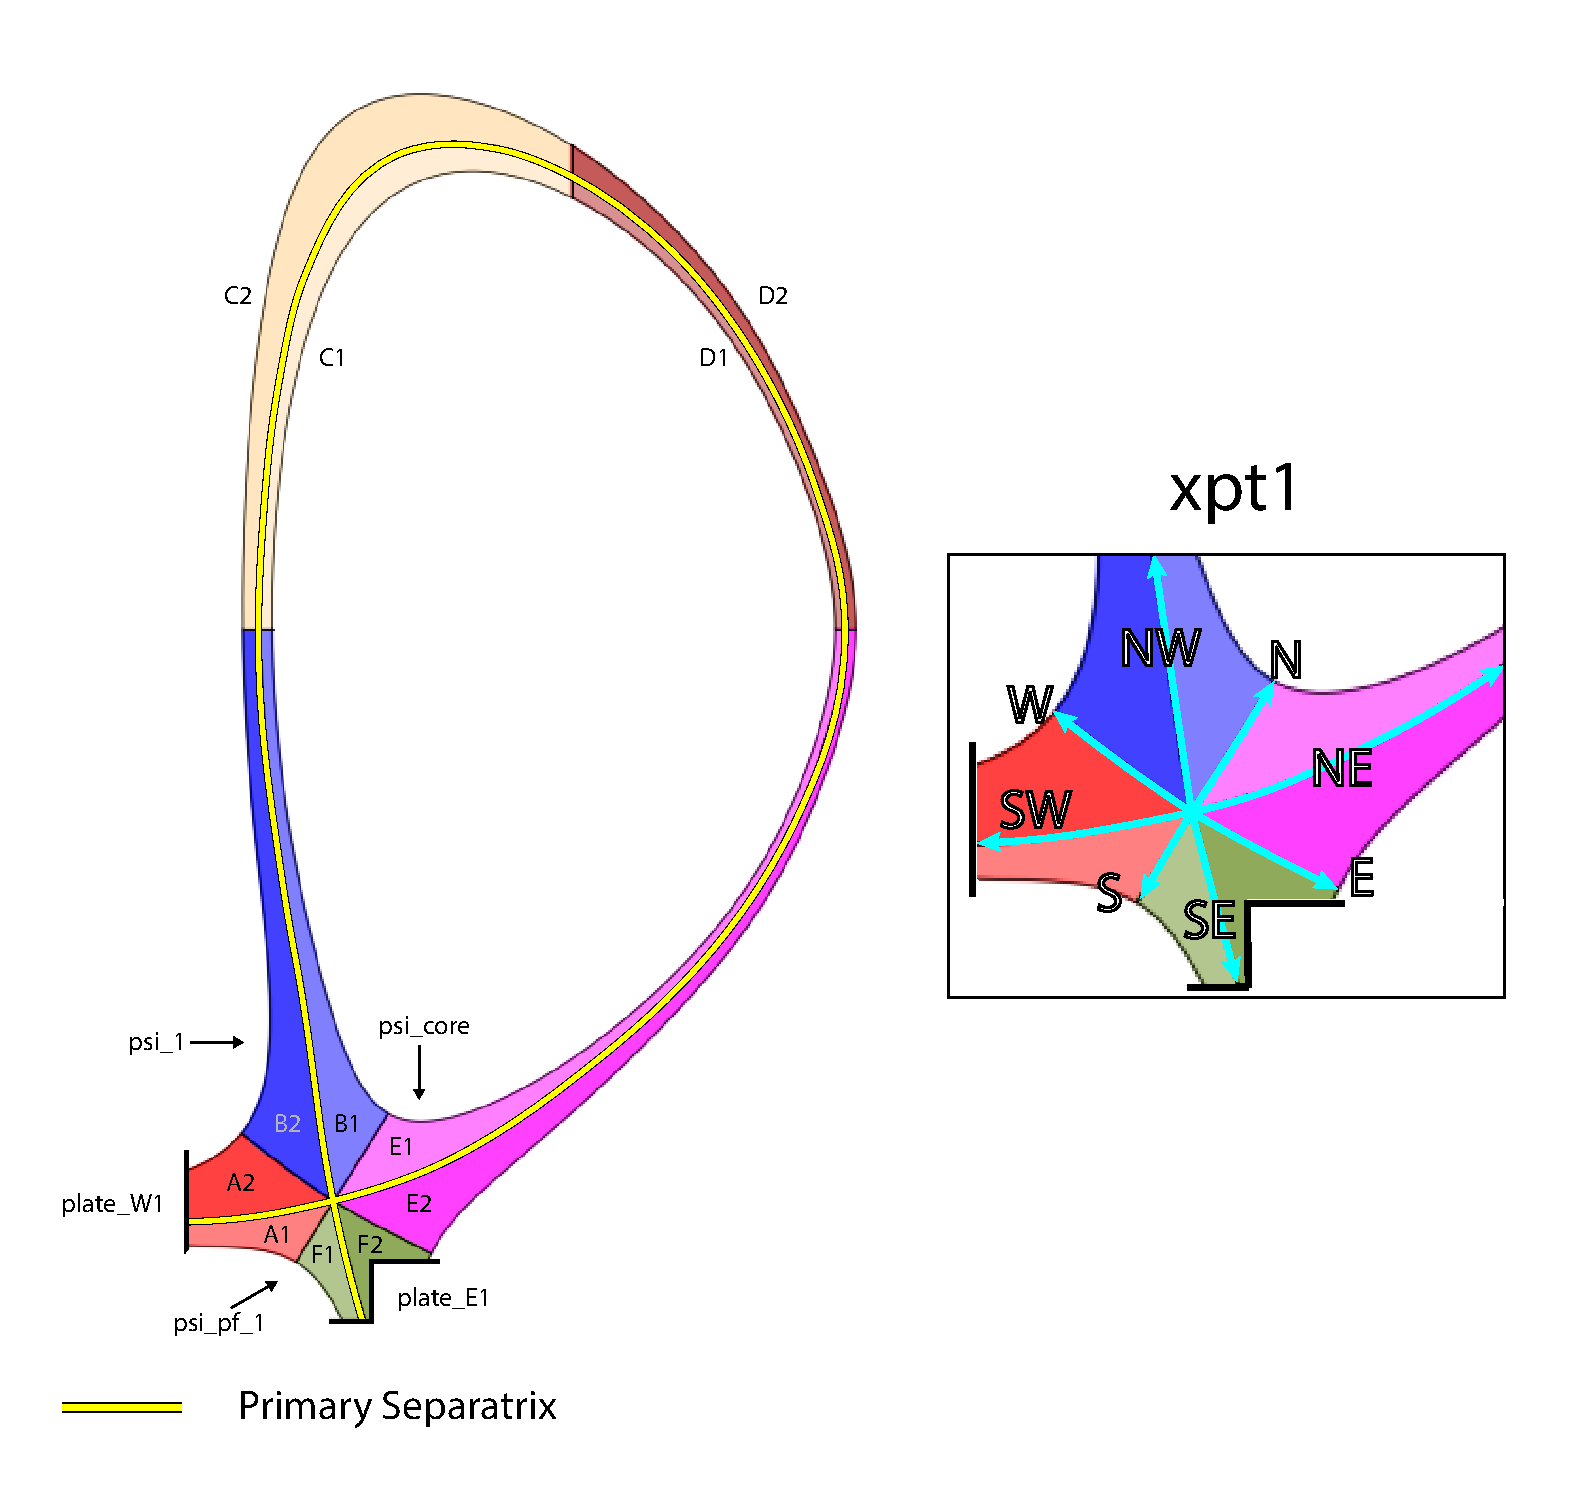
\includegraphics[width=\linewidth]{figures/xpt_1_directions.pdf}
    \caption{An SNL divertor configuration illustrating the primary x-point's N-S-E-W labeling convention.}
    \label{fig:xpt_1_directions}
\end{figure}
%\subsection{\label{sec:level2}Two x-points}
For understanding the N-S-E-W convention of the secondary x-point, it is useful to consider the partition of the domain induced by any given separatrix. With these distinct regions in mind, we define N for the secondary x-point to be the in the direction of the region that contains the primary separatrix. We assign a Point object for this N direction some $\varepsilon$ distance away from the secondary x-point. The remaining secondary x-point directions (S, E, W, SE, SW, NE, NW) are obtained by the appropriate rotations of the established N Point.\\ \indent
This secondary x-point N-S-E-W criteria is not only a critical step for identification of a divertor configuration, but also provides a general plate naming scheme for all magnetic topologies. Just like the primary x-point case, we have the ``SW" and ``SE" directions of the secondary x-point intersect individual target plates. We can see this idea and the ideas discussed earlier in figure \ref{fig:xpt_2_directions}. To remain consistent with the primary x-point target plate naming scheme, we refer to these plates as ``plate\_W2" and ``plate\_E2" for the ``SW" and ``SE" directions respectively. The ``2" here indicates that these plates are unique to the cases with two x-points.
\begin{figure}[H]
    \centering
    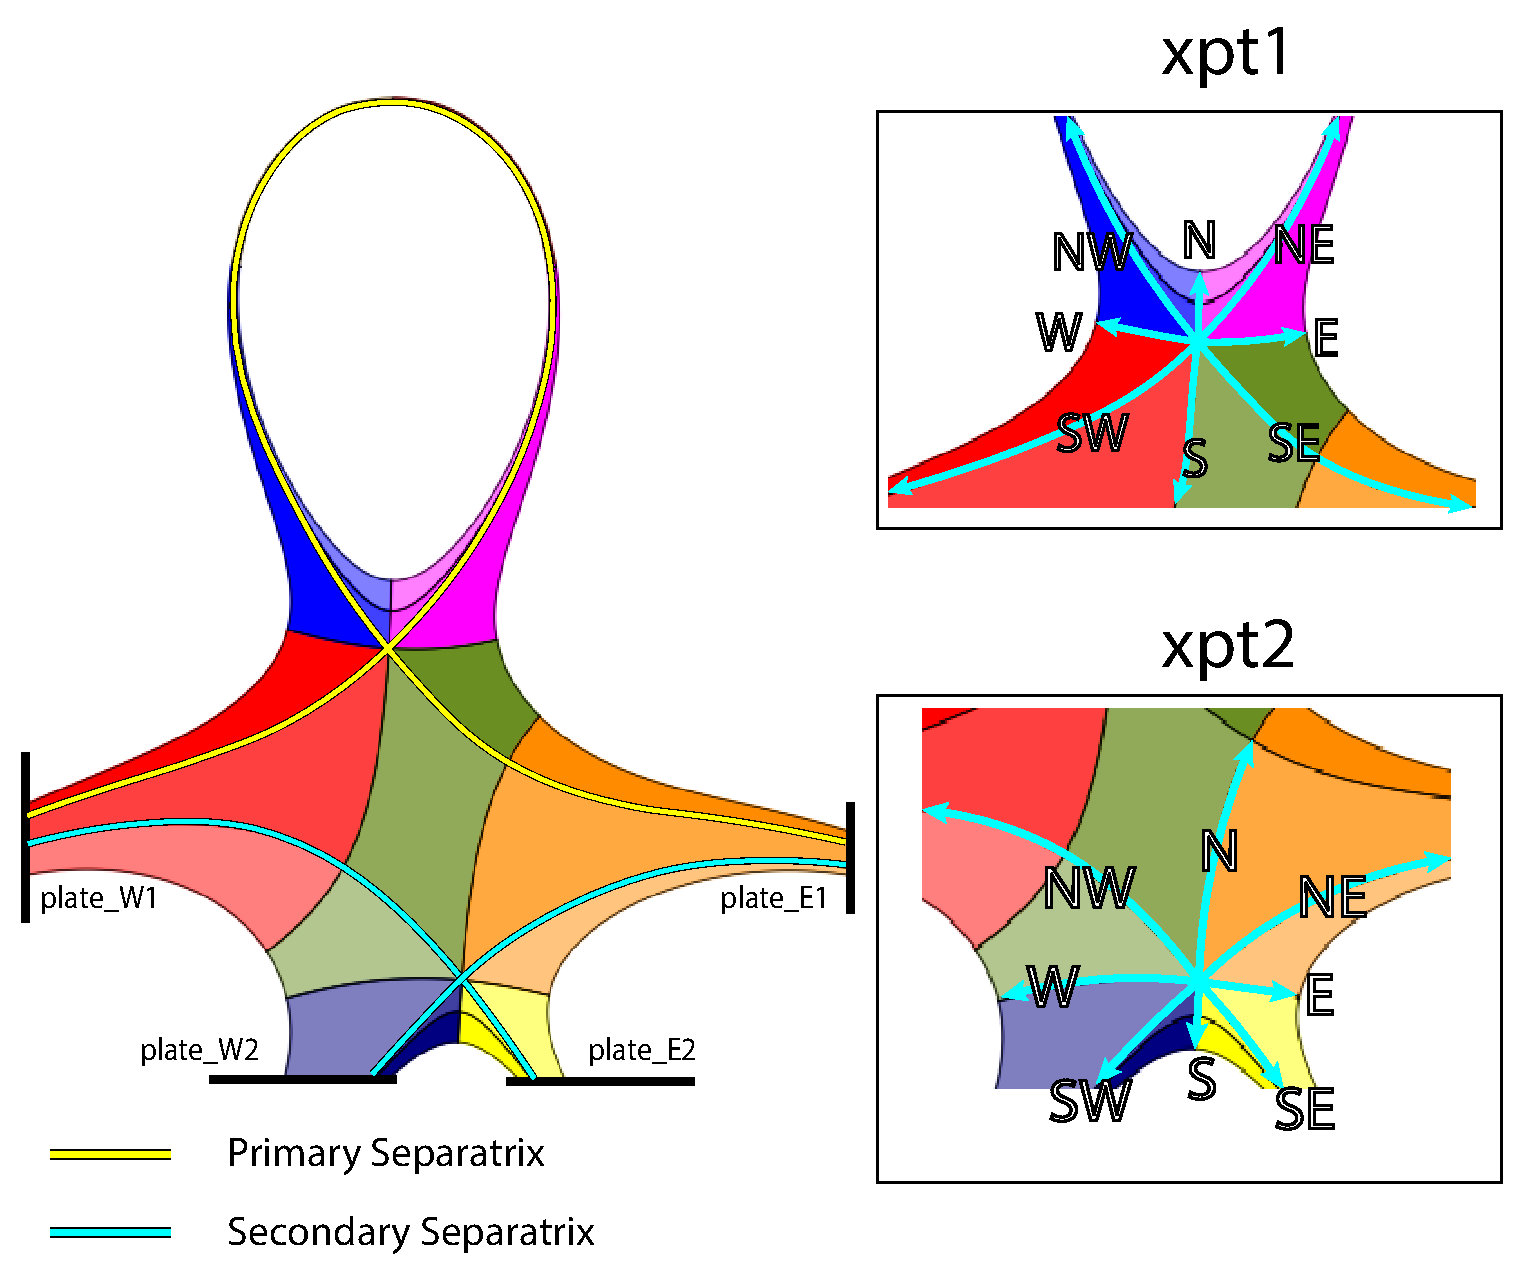
\includegraphics[width=\linewidth]{figures/xpt_2_directions.pdf}
    \caption{An SF75 divertor configuration illustrating the primary x-point and secondary x-point N-S-E-W labeling convention.}
    \label{fig:xpt_2_directions}
\end{figure}
%\subsection{Index space layout}

\section{\label{sec:level3}Computational algorithm methodology}
\subsection{\label{sec:level2} ``Divide and conquer'' strategy}

The INGRID workflow includes two main steps: (i) constructing a
``skeleton grid'' (also called further a ``patch-map'') which
corresponds to the geometry of the magnetic field in hand and consists
of a small number of quadrilateral patches; and (ii) putting a subgrid
on each of the patches. This is illustrated in
Fig. (\ref{fig:patchmap_subgrid}) where a patch-map is shown with one
of the patches covered with a subgrid.

The skeleton grid is constructed as a smallest possible grid to be
aligned with the given magnetic field and respecting the magnetic
field topology. The geometry of magnetic flux surfaces, in particular
the X-points and the magnetic axis, and the geometry of plasma facing
material surfaces all together define a patch map. For calculating a
subgrid, the code divides each quarilateral patch into a number of
radial and poloidal zones according to user-provided input. Finally,
all subgrids are joined together to produce the global grid.

\subsection{\label{sec:level2}Bicubic interpolation}
INGRID utilizes bicubic interpolation for obtaining psi values between the provided data points of a provided magnetic equilibrium eqdsk input file (EFIT file). This choice of interpolation is robust and provides us the accuracy required for modeling divertor configurations with small poloidal magnetic field values and low neqdsk resolution. The Bicubic class is composed with the EfitData class: a class responsible for the management of EFIT data provided to INGRID. With this interpolated data, INGRID is able to utilize ODE integrators to compute radial and poloidal lines. We refer to radial lines to be perpendicular to psi-surfaces, and poloidal lines to be the psi-surface contours themselves. INGRID currently utilizes scipy.integrate.LSODA for all integration purposes.

\subsection{\label{sec:level2}Line tracing}
The generation of Line objects from interpolated EFIT data is handled by INGRID's LineTracing class. A powerful feature of the LineTracing class is it's ability to determine intersection with a Line object on the fly. This is heavily utilized during the drawing of a Patch map as we often check for intersection with psi surfaces, target plates, or other Lines created by the LineTracing class. LineTracing class offers not only computational tools, but also visual tools that aid in the modeling process. We refer the interested reader can refer to the INGRID documentation available online.
\subsection{Refining reference points}
 INGRID computes high-accuracy $(r, z)$ coordinates for the magnetic-axis and X-points of interest based off the user's initial $(r, z)$ guess. Since the magnetic-axis and X-points locally represent a paraboloid and hyperbolic-paraboloid respectively, ``refined" $(r, z)$ coordinates for the magnetic-axis and X-points can be obtained by applying a root-finder to the gradient of the $\Psi$ function obtained from interpolated MHD equilibrium data. The initial guess for the root-finder is provided either via the INGRID parameter file or via command-line when not operating in GUI mode. These refined reference points are essential to key steps of the INGRID algorithm such as computing normalized $\Psi$ data, topology analysis, line-tracing, and exporting the grid. Refinement of topological reference points occurs automatically via GUI mode, but users are able to update entries interactively and on the fly should discrepancies be seen in the plot of MHD equilibrium data.
\subsection{Topology analysis}

Based on the user input, INGRID seeks a configuration with either one
or two X-points in the domain. If one X-point is required, this is a
single-null (SNL) configuration. Although in the tokamak edge plasma
community it is common to distinguish the ``upper single null'' and
the ``lower single null configurations'', for INGRID there is no
distinction between those. Instead of using ``lower'' and ``upper''
for the divertor, and ``inner'' and ``outer'' for target plates,
INGRID uses the notion of the ``compass'' directions
North-South-East-West associated with the primary X-point, and the
North direction is defined to point into the core plasma along the
$\grad \Psi$ direction. Then for a single-null configuration, one of
the plates is in the South-West direction (denoted as a ``West''
plate, and the other one is in the South-East direction, and is
denoted as the ``East'' plate, as illustrated in Fig. (\ref{fig:snl_patch_map}).

If two X-points are required to be in the domain, INGRID performs
further analysis to see in which category the given magnetic
configuration falls. First, it determines whether the secondary
X-point is in the private-flux region or in the common-flux region
(SOL) with respect to the primary separatrix. Next, an orthogonal
projection is constructed from the secondary X-point to the primary
separatrix. If the secondary X-point is in the private-flux region
with respect to the primary separatrix, this can be either SF105 or
SF75 configuration.  Then an orthogonal projection is constructed from
the secondary X-point to the primary separatrix, and based on the
location of this projection the specific configuration is identified.

In case the secondary X-point is in the common-flux region with
respect to the primary separatrix, and the secondary X-point and the
primary X-point are on opposite sides of the midplane (the horizontal
plane through the magnetic axis) this is the unbalanced double null
(UDN) configuration, see Fig. (\ref{fig:udn_patch_map}).

In case the secondary X-point is in the common-flux region with
respect to the primary separatrix, and the secondary X-point and the
primary X-point are on the same side of the midplane this can be on of
four possible cases: SF15, SF45, SF135, or SF165 configurations, see
Figs. (\ref{fig:all_conf}, \ref{fig:sf15_patch_map}-\ref{fig:sf165_patch_map}). 
An orthogonal projection is then constructed from the
secondary X-point to the primary separatrix, and based on the location
of this projection the specific configuration is identified.

%%\subsection{Handling of target plates}
INGRID users must specify the geometry of the limiter and/or target plates, to represent the shape of material walls in a modeled device. The limiter and target plates are represented in INGRID by a piecewise-linear model defined by a set of nodes; the (r,z) coordinates of those nodes are expected to be provided in separate data files. There is one data file for the limiter and one for each target plate, either in the text format or as a NumPy binary. The names of those data files are set in the INGRID parameter file. In the case that the limiter and target plate data are provided in text format, the user must specify (r,z) coordinates for each point defining the surface sequentially on a separate line in the corresponding data file; and Python-formatted single- line comments can be included, as shown in the Appendix.
For use of NumPy binary files, users must also adhere to a particular internal file structure. Given two NumPy arrays of shape $(n, )$ that represent $r$ and $z$ coordinate values respectively, one can define a NumPy array of shape $(2,n)$ representing the $n$-many points required to model the piecewise-linear model of interest. This NumPy array of shape $(2, n)$ can be saved into a NumPy binary file in order to be loaded into INGRID.
In addition to the requirements above, INGRID asserts that strike-point geometry files used for Patch maps are monotonic in psi along the length of the target plates (i.e. no shadow regions). This assertion allows for INGRID generated Patch maps to conform entirely to a user's specified strike-point geometry. While operating INGRID in GUI mode, users will be warned if the loaded geometry file is not monotonic in psi along the target plate length. 
\subsection{Construction of Patch maps}
For a given divertor configuration of interest, INGRID creates a Patch map: the collection of Patch objects that form a partition of the magnetic-topology to be modeled. Construction of a Patch map occurs after topology analysis and, upon completion, enables grid generation. INGRID takes the result of topology analysis to instantiate the appropriate topology class object that contains a collection of configuration-specific line tracing method calls for the construction of the Patch map. The newly constructed object  utilizes user provided psi-boundary values, refined topological reference points, N-S-E-W directions, and target-plate/limiter geometry to construct the final Patch map. Construction of the Patch map relies on the LineTracing class to generate the Line objects that are then trimmed, split, re-ordered, and joined together to define the appropriate Patch objects. Although line tracing routines are magnetic topology specific, there is a general approach taken to construction of Patch map.\\
First, tracing of the primary-separatrix is completed by using N-S-E-W directions obtained from x-point analysis. This is done by line tracing from xpt\_1 NW, NE, SW, and SE. Line tracing from the NW and NE directions form the ``loop" around the core-region, and line tracing originating from the SW and SE directions form the ``legs" of the seperatrix and terminate upon intersection with the appropriate user provided strike point geometry (target-plates or limiter). \\
After tracing of the primary-separatrix, line tracing continues from xpt\_1 with starting points in the N, S, E, W directions and termination occurring upon intersection with the magnetic-topology dependent psi-boundary level provided by the user. The Patch map figures illustrate this configuration dependence. Tracing in the N, S, E, or W direction to a new psi-level enables poloidal line tracing to continue on a new psi-level. This stage in the line tracing is repeated until all Patch boundaries are formed. These boundaries can be seen in the Patch map diagrams provided. Generating a Patch map in the case of two x-points follows the same general framework with the addition of secondary-separatrix line tracing.
\subsection{Grid construction}

For a given magnetic configuration, a Patch-Map represents a very
crude grid where each Patch is a ``quadrilateral'' with four vertices.
The radial sides of this quadrilateral are defined by two flux
surfaces, $\Psi(R,Z)=\Psi_1$ and $\Psi(R,Z)=\Psi_2$. The poloidal
sides of a Patch are usually constructed to be aligned with $\nabla
\Psi$, which makes the skeleton grid locally orthogonal. 

However, more generally the poloidal sides of a Patch can deviate from
the $\nabla \Psi$ direction. For example, for those patches that
contain the poloidal boundaries of the domain, given by the target
plates, one of the sides is defined by the target plate shape. The
curve describing the target plate can be arbitrary, as long as it does
not form ``shadow regions'', i.e., $\Psi$ is a continuous function of
the length along the plate.

Going beyond the skeleton grid, a Patch can be divided in a number of
radial and poloidal zones, forming a subgrid local to this patch. The
radial zones are constructed to be aligned with flux surfaces, so the
global grid remains aligned with the poloidal magnetic field. For the
poloidal zones, the main algorithm is based on dividing the patch
poloidally into equal size segments. However, as described further,
there are options in the code for controlling the radial and poloidal
distribution of subgrid.

The radial and poloidal dimensions and distribution of subgrid on a
given Patch are not entirely independent of subgrids on other patches
as the global grid still has to be Cartesian in the index space. Thus
the poloidal grid has to be consistent for those patches that are
stacked on top of each other radially, and the radial grids have to be
consistent for those patches stacked on top of each other poloidally.

\subsection{Customization of grids}
INGRID provides users tools for customization of generated grids that can be controlled via the parameter file. Patch map modification and grid modification the two approaches to grid optimization.\\ \indent
Default Patch map settings can be configured before configuration specific line tracing scripts are run. Modification of Patch map settings allow the user to influence the resultant regions of the computational domain to be modelled. User settings available for specification currently consist of magnetic-axis translation and midplane orientation adjustment.\\ \indent
INGRID utilizes the refined magnetic-axis coordinates as a reference point for line tracing termination criteria by searching for intersection with horizontal and vertical lines that emanate from the magnetic-axis. Patches whose E/W boundaries are defined by vertical and horzontal lines through the magnetic-axis are adjusted by applying an $(r,z)$ translation to the reference coordinates of the magnetic-axis. INGRID also allows users to rotate the vertical and horizontal lines about the magnetic-axis coordinates. These rotation values are specified in the INGRID parameter file.\\ \indent
Patch refinements settings for the resultant grid can be specified in the parameter file in a similar manner to Patch map modifications. Features for resultant grids can be specified on a per Patch basis and include $\text{np}\times\text{nr}$ grid dimension specification, poloidal distribution transformations, radial distribution transformations, and automatic shearing correction for increasing orthogonality in heavily-sheared regions of a grid.\\ \indent
The Patch map system introduced allows for users to specify grid settings on a per-Patch basis by assigning ``Patch tags": a two character, alphanumeric string with the first character (strictly-alpha) referring to poloidal ``column" in index-space, and second character (strictly-numeric) referring to a radial ``row" in index-space. Using the Patch map naming system, users can specify grid dimensions for specific regions in an index-space consistent manner. Setting the poloidal np grid dimension in Patch objects A2 and A1 to a value of 10 is done by specifying ``np\_A: 10" in the parameter file. Because Patch objects A2 and A1 are adjacent poloidally, INGRID only needs the user to refer to the alpha character ``A" for the setting of poloidal np grid dimension. To adjust the radial nr resolution for the private-flux region to a value of 10, users specify ``nr\_1: 10" in the parameter file. When no Patch specific grid dimension settings are provided for a Patch, ``np\_default" and ``nr\_default" values are utilized.\\ \indent
During Patch refinement, grid seed-points are distributed uniformly in length along N/S Patch boundaries and distributed uniformly along E/W Patch boundaries in locally-normalized psi. This default behavior can be changed so that grid seed-point placement obeys a user specified distribution function. For specifying distribution/transformation functions, users provide a string in the parameter file that takes the form ``$x, f(x)$" with $f$ being the distribution/transformation function of interest, and $x \in [0, 1]$ acting as the parameterization variable along a Patch boundary. INGRID requires the user specified distribution function to satisfy $\text{range}(f) \in [0, 1]$. This is a result of N/S Patch boundaries being normalized in length and E/W Patch boundaries being locally-normalized in psi. Following this convention, it can be seen that INGRID's default uniform distribution follows the rule ``$x,\,x$``. INGRID utilizes the SymPy\cite{10.7717/peerj-cs.103} package to generate a lambda function from the user provided string.
The SymPy backend supports functions that conforms to standard Python arithmetic operations (*, **, etc), and common functions such as ``exp", ``log", ``sin", and ``cos". The user provides all grid transformations in the parameter file and can specify transformations on a per-Patch basis via the Patch tag naming convention. Modifying the uniform poloidal distribution in Patch objects A2 and A1 to follow a $\sqrt{x}$ distribution is done by specifying ``poloidal\_f\_A: x, x ** (0.5)" in the parameter file. Similarly, to modify the uniform radial distribution for the private-flux region to follow the same $\sqrt{x}$ rule, the user must specify ``radial\_f\_1: x, x ** (0.5)" in the parameter file.\\ \indent
INGRID provides users the ``\texttt{distortion\_correction}" tool in order to mitigate grid shearing that occurs in a produced grid. The \texttt{distortion\_correction} tool works by allowing the user to specify constraints on the corner angles formed in Cell objects that form the mesh. These constraint variables are referred to as ``theta\_min" and ``theta\_max" in the parameter file and define the angle threshold for a Cell. During Patch refinement, INGRID will shift the generated Cell vertex by increments of $\frac{1}{dr}$ until the resultant angle is within the user constraints. This $dr$ value is the inverse of a ``resolution" variable specified by the user in the parameter file. If the constraint cannot be satisfied (vertex leaves the Patch), INGRID will backtrack until the vertex is within the Patch bounds. An example of the \texttt{distortion\_correction} feature applied to a grid can be seen in figure \ref{fig:distortion_correction}.

\section{\label{sec:level5}Performance}
\subsection{Scaling of calculation time}

The results of INGRID timing test on a MacBook computer are shown in
Table (\ref{benchmark_table_1}) and in
Fig. (\ref{fig:benchmark_grid_scaling}). The scaling appears sublinear
for small grids; for larger grids it asymptotes to linear. Note that
the cost of grid generation is not significant in a typical edge
plasma modeling workflow; running the simulation takes orders of
magnitude more computing time.\\

\begin{tabular}{|c|c|c|}
    \toprule
    \multicolumn{3}{|c|}{SNL}\\
    \cline{1-3}
    {Cells Per Patch} & Total Cells &    Time (s) \\
    \midrule
    9  &       108 &   48.321923 \\
    16  &       192 &   63.920347 \\
    25  &       300 &   82.622279 \\
    36  &       432 &  100.041368 \\
    49  &       588 &  118.413244 \\
    64  &       768 &  138.113504 \\
    81  &       972 &  153.613585 \\
    100  &      1200 &  171.291218 \\
    121  &      1452 &  189.555594 \\
    144  &      1728 &  198.343664 \\
    169 &      2028 &  215.742957 \\
    196 &      2352 &  236.941801 \\
    225 &      2700 &  250.419288 \\
    \bottomrule
\end{tabular}

\begin{tabular}{|c|c|c|}
    \toprule
    \multicolumn{3}{|c|}{SF75}\\
    \cline{1-3}
    {Cells Per Patch} & Total Cells &   Time (s) \\
    \midrule
    9  &       243 &   73.644410 \\
    16  &       432 &   99.189812 \\
    25  &       675 &  127.370058 \\
    36  &       972 &  155.958905 \\
    49  &      1323 &  181.518565 \\
    64  &      1728 &  206.474669 \\
    81  &      2187 &  230.737183 \\
    100  &      2700 &  253.775640 \\
    121  &      3267 &  281.557351 \\
    144  &      3888 &  305.958863 \\
    169 &      4563 &  332.568824 \\
    196 &      5292 &  359.910149 \\
    225 &      6075 &  387.905040 \\
    \bottomrule
\end{tabular}
\label{benchmark_table_1}
\subsection{Benchmark testing}

To verify grids calculated by INGRID, several benchmark tests have
been performed with the UEDGE code.

In these testes, UEDGE solutions were compared, using grids from
INGRID and grids produced with the UEDGE internal grid generator; for
the same physics problem statement, the same boundary conditions,
using the same (or very close) domain geometry.

In one of these test problems, a snowflake-like SF75 configuration was
used, based on magnetic reconstruction data from the TCV tokamak. The
UEDGE grid generator cannot deal with the SF75 configuration directly;
but it can be set up to treat each X-point as a part of a separate SN
configuration, and then joining two such SN grids together one can
produce a grid for the full SF75 domain.

The UEDGE code was set up to solve to the steady state the
time-evolution equations for plasma density, plasma parallel momentum,
ion thermal energy, and electron thermal energy.


\beq
%
\pdiff{}{t} n_i + \grad \cdot 
\left[ n_i \vec{V}_i \right]
= S_i \\
%
\eeq

\beq
\pdiff{}{t} \left[ M n_i {V}_{i,||} \right] + \grad \cdot
\left[
M n_i \vec{V}_i {V}_{i,||}  - \hat{\eta}_i \grad {V}_{i,||}
\right]
= S_{m,||}
\eeq

\beq
\pdiff{}{t}
\left[
\frac{3}{2} n T_i
\right]
+
\grad \cdot
\left[
\frac{5}{2} n_i T_i \vec{V}_i
+
\vec{q}_i
\right] = S_{E,i}
%
\eeq

\beq
\pdiff{}{t}
\left[
\frac{3}{2} n T_e
\right]
+
\grad \cdot
\left[
\frac{5}{2} n_e T_e \vec{V}_e
+
\vec{q}_e
\right] = S_{E,e}
%
\eeq

Here we use the standard notation: $n_i$ is the plasma density,
$\vec{V}_i$ is the plasma fluid velocity, $T_{e,i}$ is the electron
and ion temperature, $\vec{q}_{e,i}$ is the electron and ion heat
flux, $S_i$, $S_{m,||}$, $S_{E,e,i}$ are sources of plasma density,
parallel momentum, and electron and ion thermal energy.

The grids used for the calculation are shown in Fig. (\ref{fig:ingrid_grid}). The
grid generated with the UEDGE grid generator is constructed to be
strictly locally orthogonal; the grid from INGRID is not
orthogonal. Also, there is slight difference in the domain
shape. Still, the steady state solutions exhibit essentially the same
distributions of plasma density, temperature, and parallel flow
velocity, as can be seen in Fig. (\ref{fig:benchmark_collection}).


\section{\label{sec:level6}Software design and user interaction}
\subsection{\label{sec:level2}Choice of development in Python}

INGRID has been exclusively developed in the Python programming
language. Python has an advantage as a free, community supported
language with extensive graphical and numerical libraries. In addition
to the developer tools readily available, the large scientific
computing user base puts INGRID in a good position for extensive use
within the edge-plasma modeling community and continued
development. Python is a choice of object-oriented programming
language that is being increasingly utilized in major tokamak plasma
modeling projects such as OMFIT \cite{Meneghini_2015,
  Orso_MENEGHINI2013} and PyUEDGE \cite{PyUEDGE}. This makes Python a
natural and consistent choice to carry out software development
needs. INGRID makes heavy use of Python's free and robust libraries in
all computational tasks, data visualization, and GUI
development. Packages such as numpy, SciPy, matplotlib, SymPy, PyYAML,
and tkinter are central developer tools utilized within the INGRID
project\cite{numpy_5725236, virtanen2019scipy,
  matplotlib_4160265, PyYAML}. Software project setup, maintenance, and
installation is easily achieved in Python through native package
structuring conventions and external package management tools such as
setuptools.  Within the INGRID package are a variety of modules
containing classes related to geometric representations, line tracing,
interpolation, and other INGRID management tasks. Two INGRID
subpackages are dedicated to GUI development and magnetic topology
modules.

\subsection{\label{sec:label2}INGRID package organization}
The top-level INGRID package includes a collection of modules responsible for the essential grid-generation processes, as well as two subpackages dedicated to the GUI and supported magnetic-topology models. Modules \texttt{ingrid} and \texttt{utils} contain classes responsible for management and execution of INGRID functionality, whereas modules \texttt{geometry}, \texttt{interpol}, and \texttt{line\_tracing} contain classes responsible for computational tasks such as topology modeling, interpolation of data, and line tracing. \\ \indent
The \texttt{Ingrid} class is contained within the \texttt{ingrid} module and is designed to provide a high-level interface for users. This \texttt{Ingrid} class is used to activate INGRID's GUI mode and also contains high-level methods for importing data, visualizing data, analyzing data, grid-generation, and exporting of data; all of which can be utilized in Python scripts. Class \texttt{IngridUtils} is contained within the \texttt{utils} module and serves as the base class for \texttt{Ingrid}. \texttt{IngridUtils} class methods encapsulate much of the lower-level software details used to implement the methods in the \texttt{Ingrid} class. Because of this, \texttt{IngridUtils} is encouraged for use by advanced users and developers of INGRID. In addition to \texttt{IngridUtils}, class \texttt{TopologyUtils} can be found within the \texttt{utils} module. In a manner similar to \texttt{IngridUtils}, the \texttt{TopologyUtils} class serves as a base class for each magnetic-topology class within the \texttt{topologies} subpackage. \texttt{TopologyUtils} contains key methods for generating Patch maps, visualizing data, generating grids, and exporting grids in gridue format. Eight magnetic-topology classes are contained within their own modules within the \texttt{topologies} subpackage: \texttt{SNL}, \texttt{UDN}, \texttt{SF15}, \texttt{SF45}, \texttt{SF75}, \texttt{SF105}, \texttt{SF135}, and \texttt{SF165}. Each magnetic-topology class contains configuration specific line-tracing instructions for construction of Patch maps, Patch map layout information, and gridue formatting information. \texttt{Ingrid} and \texttt{IngridUtils} conduct analysis of MHD equilibrium data in order to decide which magnetic-topology class to instantiate from the \texttt{topologies} subpackage. The \texttt{IngridUtils} class always maintains a reference to the instantiated object in order to effectively manage grid-generation.\\ \indent
All GUI operation is managed by class \texttt{ingrid\_gui} within the \texttt{gui}s subpackage. INGRID's GUI front-end was developed with the tkinter package; a Python interface to the Tk GUI toolkit that is available within the Python Standard Library. Class \texttt{ingrid\_gui} is simply responsible for managing event handling, and managing an \texttt{Ingrid} object that is used to drive the GUI with direct calls to the available high-level methods.\\ \indent
Beyond modules \texttt{ingrid} and \texttt{utils}, modules \texttt{geometry}, \texttt{interpol}, and \texttt{line\_tracing} form the computation and modeling foundation of INGRID. Classes \texttt{Bicubic} and \texttt{EfitData} can be found within the \texttt{interpol} module. The \texttt{Bicubic} class handles biciubic interpolation of data and is composed with classes that directly utilize bicubic interpolation. Class \texttt{EfitData} is used to provide an interpolated representation of provided MHD equilibrium data. \texttt{EfitData} computes partial derivative information of MHD equilibrium data, provides interpolated $\psi$ function values by interfacing with class \texttt{Bicubic}, and contains methods for visualisation of interpolated MHD equilibrium data. Module \texttt{geometry} contains classes \texttt{Point}, \texttt{Line}, \texttt{Patch}, and \texttt{Cell}. These classes are the building-blocks for creation of Patch maps and generation of grids.
\subsection{\label{sec:label2}INGRID geometry object hierarchy}
If we are to adopt an object-oriented approach to grid generation, then we must develop a set of tools that can be utilized throughout our project. Here we discuss how INGRID defines a collection of geometric classes in order to make the grid generating process as simple as possible for all magnetic topologies of interest. To do so, INGRID defines the following collection of geometric abstractions: the Point class, the Line class, the Cell class, and the Patch class. All together, these classes arm INGRID with the ability to represent any magnetic topology of interest. We provide a very brief description of the classes here. Figure \ref{fig:patchmap_subgrid} illustrates the geometry collection described below.\\
\indent
A Point object simply represents an arbitrary $(r,z)$ spatial coordinate. A Line object object is defined by two or more Point objects. This Line object definition allows for the representation of any arbitrary curve we may encounter (e.g. psi-surface, target plate, limiter geometry). A Patch object represents a quadrilateral region of the domain. Patches are defined by four Line objects. This Patch abstraction allows for partitioning of the domain of interest into various regions that we would like to obtain a grid representation of. A Cell object resides within a Patch and represents a quadrilateral grid cell. Cells are defined by five Point objects: four corners and a center. These Cell objects contain spatial and experimental data that are to be used in simulation code.\\ \indent
From these definitions, we have the building blocks for modeling any of the magnetic topologies of interest we mentioned in the previous section. In particular, we aim to construct a collection of Patch objects representing the divertor configuration of interest. We call this collection of Patch objects a Patch map. This Patch map allows us to create a grid of Cell objects within each Patch, thus providing the final grid. The management of the Patch map creation and grid generation is managed by a magnetic topology class of modeling interest. \\ \indent
As of the current INGRID release, we have defined magnetic topology classes SNL, UDN, SF15, SF45, SF75, SF105, SF135, and SF165. These are contained within a dedicated topologies subpackage within the INGRID code. We also introduce a general ``Ingrid" class exclusively meant for user interfacing and management. The Ingrid class and all magnetic topologies are supported by the backend utility classes IngridUtils and TopologyUtils respectively. We will discuss these classes at a later part of the report.

\subsection{\label{sec:level2}The INGRID parameter file}
INGRID has been designed to be controlled from a single configuration/parameter file when operating in GUI mode. We have decided to use YAML formatted files for the parameter file\textbf{[CITE YAML]}. This YAML file is similar to the familiar Fortran namelist files due to the key-value structure it is based off of. YAML is in an easy to read format that has extensive support within Python. With the PyYAML library, Python reads a YAML formatted file and internally represents it as a Python dictionary. This allows users to model cases in the INGRID GUI and reuse a parameter file in scripting for later usage (e.g. batch grid generation). Some key controls within the parameter file include: EFIT file specification, specification of number of x-points, approximate coordinates of x-point(s) of interest, approximate magnetic-axis coordinates, psi level values, and target plate settings (files, transformations). Other controls in the parameter file include: path specification for data files, grid cell np/nr values, poloidal and radial grid transformation settings, limiter specific settings, saving/loading of Patch maps, gridue settings, and debug settings. This is not an exhaustive list. Further details can be found in INGRID's Read The Docs online documentation. Section A in the appendix shows a small snippet of an INGRID parameter file for an SNL case. 
\subsection{INGRID target plate file}

INGRID users must specify the geometry of the limiter and/or target
plates, to represent the shape of material walls in a modeled
device. The limiter and target plates are represented in INGRID by a
piecewise-linear model defined by a set of nodes; the (r,z)
coordinates of those nodes are expected to be provided in separate
data files. There is one data file for the limiter and one for each
target plate, either in the text format or as a NumPy binary. The
names of those data files are set in the INGRID parameter file. In the
case that the limiter and target plate data are provided in text
format, the user must specify (r,z) coordinates for each point
defining the surface sequentially on a separate line in the
corresponding data file; and Python-formatted single- line comments
can be included, as shown in the Appendix.

For use of NumPy binary files, users must also adhere to a particular
internal file structure. Given two NumPy arrays of shape $(n, )$ that
represent $r$ and $z$ coordinate values respectively, one can define a
NumPy array of shape $(2,n)$ representing the $n$-many points required
to model the piecewise-linear model of interest. This NumPy array of
shape $(2, n)$ can be saved into a NumPy binary file in order to be
loaded into INGRID.  In addition to the requirements above, INGRID
asserts that strike-point geometry files used for Patch-Maps are
monotonic in psi along the length of the target plates (i.e. no shadow
regions). This assertion allows for INGRID generated Patch-Maps to
conform entirely to a user's specified strike-point geometry. While
operating INGRID in GUI mode, users will be warned if the loaded
geometry file is not monotonic in psi along the target plate length.

\subsection{\label{sec:level2}INGRID workflow}
INGRID can be operated via GUI or utilizing the INGRID library directly in Python scripts. The GUI workflow highlights the interactive nature of INGRID by allowing users to visually inspect MHD equilibrium data, configure geometry, and refine parameter file values on the fly. For both GUI operation and scripting with INGRID, the high-level INGRID workflow is: (i)  Parameter file visualization and editing, (ii) Analysis of MHD equilibrium data and creation of Patch map, (iii) Patch map refinement and gridue export.
\noindent
INGRID internally handles step (ii) and leaves the user to with steps (i) and (iii). These steps are where the user is able to customize the Patch map and grid to meet their modeling needs.\\ \indent
Step (i) in the INGRID workflow allows users to visually inspect MHD equilibrium data, target-plates \& limiter geometry, and psi-level contours that are specified within a loaded parameter file. Since creation of grids is tied directly to MHD equilibrium analysis and Patch map creation, step (i) is crucial for successful grid generation. To simplify this step, the INGRID GUI provides an easy to use workspace for preparation of a parameter file for the subsequent analysis of MHD equilibrium data and Patch map creation. Examples of common operations at this step include modifications to strike-point geometry and psi-level boundaries for subsequent Patch maps. Once a user is satisfied with parameter file settings, step (ii) can be immediately executed with no further user intervention. Should any errors in Patch map creation occur (e.g. misplaced target-plates, psi-boundaries that do not conform to configuration specific requirements), INGRID will prompt the user and allow for appropriate edits to be made. Upon completion of step (ii), the created Patch map will be provided to users as a new matplotlib figure. From here the user can decide to proceed with Patch map refinement or start over at step (i) to make edits to the Patch map.\\ \indent
In order to streamline grid generation and skip directly to step (iii), INGRID supports Patch map reconstruction. This feature allows users to bypass line-tracing routines by reloading a saved Patch map from a previous INGRID session. To do so, INGRID encodes essential geometry and topology analysis data in a specially formatted dictionary that is then saved as a NumPy binary file. Class \texttt{IngridUtils} handles the encoding and reconstruction of Patch maps. These reconstruction features can be configured by the user within the INGRID parameter file.\\ \indent
After a Patch map has been generated or reconstructed, users can configure grid generation specific settings that will be utilized during Patch map refinement. Similar to Patch map generation, once all local subgrids have been created within Patch objects, a new matplotlib figure is presented with the generated grid. From here, users can make grid generation setting edits in the INGRID parameter file or proceed to exporting a gridue file.
% \subsection{\label{sec:level2}Obtaining and running INGRID}
% INGRID is currently available for download on Github and extensive documentation has been prepared for both installation and running of the code. We refer the interested reader to our online INGRID Read The Docs.

\section{\label{sec:level7}Summary}
\subsection{\label{sec:level2}Summary}
INGRID is a new grid generator for tokamak boundary region, it is
capable of producing grids for single-null (SNL), unbalanced
double-null (UDN), and snowflake-like (SF) configurations. Currently,
exported grids are in the format of the UEDGE code, and future
development anticipates the addition of additional formats as adoption
of INGRID increases in the broader edge-plasma community. INGRID can
be utilized via the INGRID Python package, or through a parameter file
driven GUI mode. The internal equilibrium file analysis algorithm
provides the ability to automatically identify the divertor
configuration embedded within experimental data with minimal user
interaction. A divide and conquer, geometry class hierarchy approach
to grid generation is at the heart of INGRID and leads to the Patch
map abstraction: a partition of the modeling domain that allows for
localized grid generation. These localized grids are combined into a
global grid that are then ready for export. Current computational
scaling of grid generation algorithm follows a sublinear trend
independent of magnetic-topology modeled. Benchmarking of INGRID
against the internal grid generator in UEDGE was conducted on an SF75
configuration. These tests illustrated INGRID's ability to both
reproduce a grid obtained with UEDGE's internal grid generator and
produce consistent UEDGE simulation results, but at a fraction of the
effort with regards to generating the grid.

\section{Acknowledgments}
The authors would like to thank M.E.Rensink for his help with grid
generation in UEDGE. This work was performed for U.S. Department of
Energy by Lawrence Livermore National Laboratory under Contract
DE-AC52-07NA27344.


\section{Appendix: Parameter file}
%\newpage
\onecolumngrid
%\section{Parameter file}
A snippet of an INGRID parameter file is shown below. Extensive documentation and tutorials for parameter file setup can be found in the INGRID Read The Docs documentation online.
\begin{lstlisting}[basicstyle=\small, aboveskip=\bigskipamount, frame=single, captionpos=b, caption={Snippet of YAML formatted configuration file. YAML files utilize Python formatted comments, keyword-value mappings, and nesting of structures via indentation.}]
# ---------------------------------------------------
# User data directories
# ---------------------------------------------------
dir_settings:
  eqdsk: ../data/SNL/DIII-D/  # dir containing eqdsk
  limiter: .  # dir containing limiter
  patch_data: ../data/SNL/DIII-D/  # dir containing patch data
  target_plates: ../data/SNL/DIII-D/ # dir containing target plates
# ---------------------------------------------------
# eqdsk file name
# ---------------------------------------------------
eqdsk: neqdsk
# ---------------------------------------------------
# General grid settings
# ---------------------------------------------------
grid_settings:
  # ----------------------------------------------------------------------------
  # Settings for grid generation (num cells, transforms, distortion_correction)
  # ----------------------------------------------------------------------------
  grid_generation:
    distortion_correction:
      all:
        active: True # true, 1 also valid.
        resolution: 1000
        theta_max: 120.0
        theta_min: 80.0
    np_default: 3
    nr_default: 3
    poloidal_f_default: x, x
    radial_f_default: x, x
  # ---------------------------------------------------
  # guard cell size
  # ---------------------------------------------------
  guard_cell_eps: 0.001
  # ---------------------------------------------------
  # num levels in efit plot
  # ---------------------------------------------------
  nlevs: 30
  # ---------------------------------------------------
  # num xpts
  # ---------------------------------------------------
  num_xpt: 1
  patch_generation:
    strike_pt_loc: target_plates # 'limiter' or 'target_plates'
    rmagx_shift: 0.0
    zmagx_shift: 0.0
  # ---------------------------------------------------
  # Psi levels
  # ---------------------------------------------------
  psi_1: 1.066
  psi_core: 0.95
  psi_pf_1: 0.975
  # ---------------------------------------------------
  # magx coordinates
  # ---------------------------------------------------
  rmagx: 1.75785604
  zmagx: -0.0292478683
  # ---------------------------------------------------
  # xpt coordinates
  # ---------------------------------------------------
  rxpt: 1.300094032687
  zxpt: -1.133159375302
  # ---------------------------------------------------
  # Filled contours vs contour lines
  # ---------------------------------------------------
  view_mode: filled
# ---------------------------------------------------
# Saved patch settings
# ---------------------------------------------------
patch_data:
  file: LSN_patches_1597099640.npy
  preferences:
    new_file: true
    new_fname: LSN_patches_1597099640.npy
  use_file: false
# ---------------------------------------------------
# Integrator
# ---------------------------------------------------
integrator_settings:
  dt: 0.01
  eps: 5.0e-06
  first_step: 5.0e-05
  max_step: 0.064
  step_ratio: 0.02
  tol: 0.005
# ---------------------------------------------------
# Limiter settings
# ---------------------------------------------------
limiter:
  file: ''
  use_efit_bounds: false
# ---------------------------------------------------
# target plate settings
# ---------------------------------------------------
target_plates:
  plate_E1:
    file: d3d_otp.txt
    zshift: -1.6
  plate_W1:
    file: d3d_itp.txt
    zshift: -1.6
\end{lstlisting}


\bibliography{ingrid_bib}
\begin{figure}[H]
    \centering
    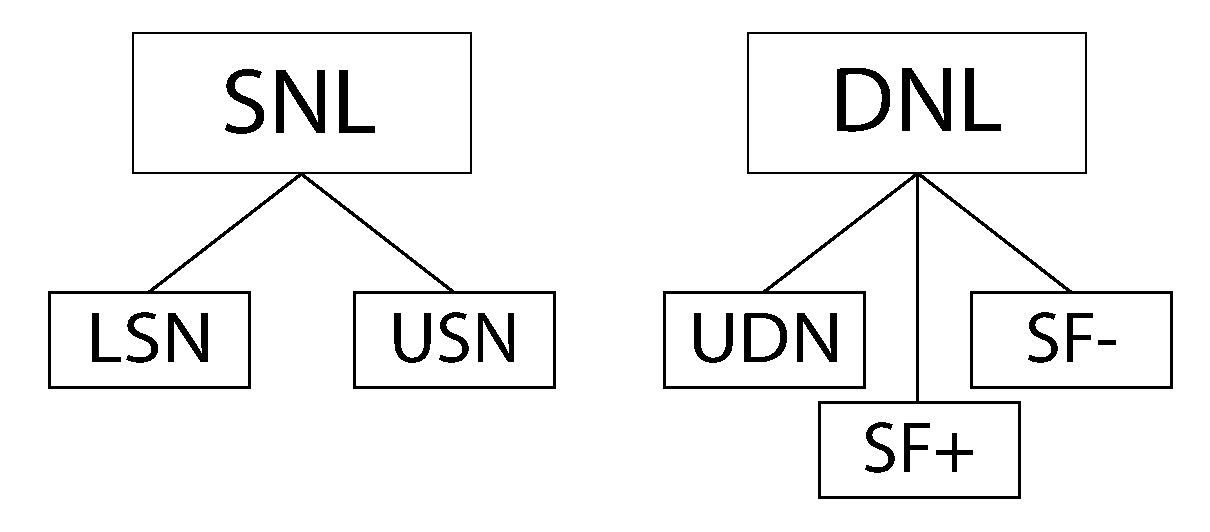
\includegraphics[width=\linewidth]{figures/config_group.pdf}
    \caption{Categorizing magnetic topologies by number of x-points induces a natural design pattern for a grid generator.}
    \label{fig:config_group}
\end{figure}

\begin{figure}[H]
    \centering
    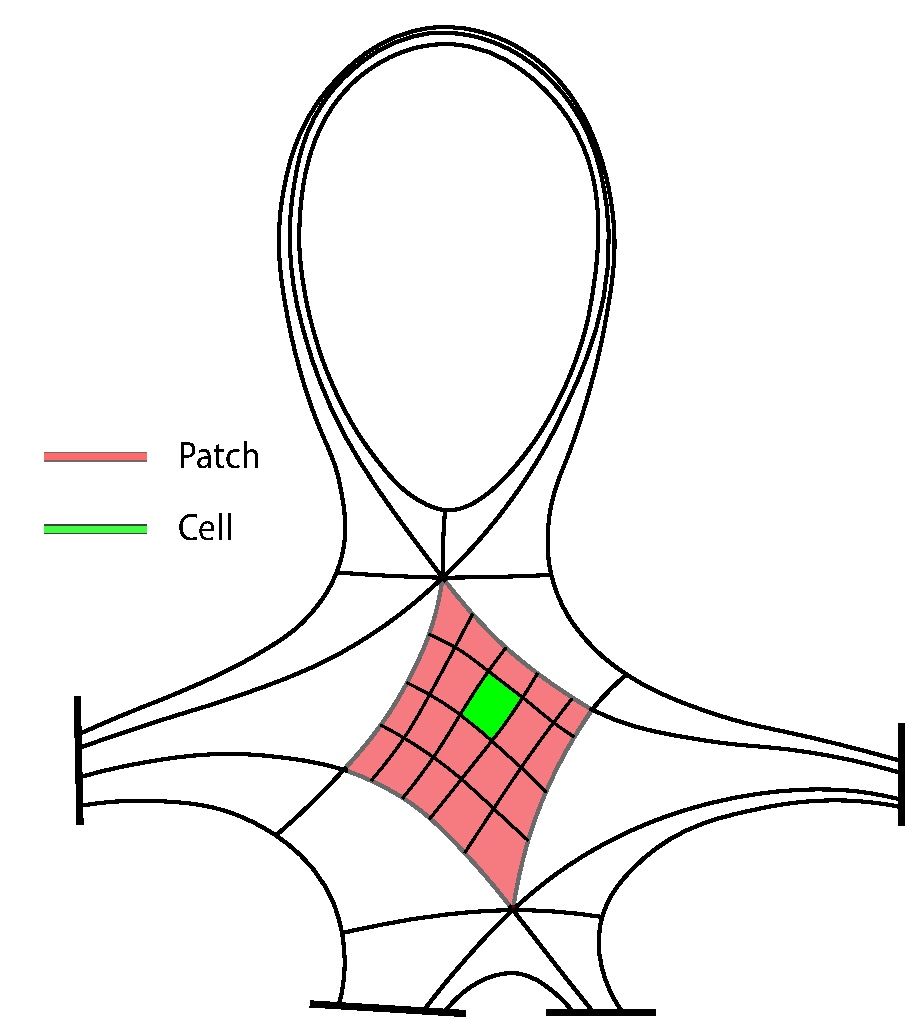
\includegraphics[width=0.35\linewidth]{figures/geometry_render.pdf}  % scale=0.35
    \caption{\label{fig:geo_collection} INGRID geometric objects are used to represent an arbitrary magnetic topology. Here we explicitly see a Patch, Cell, and Line. Points are implicitly shown by a Line and Cell object definition.}
\end{figure}

\begin{figure}[H]
    \centering
    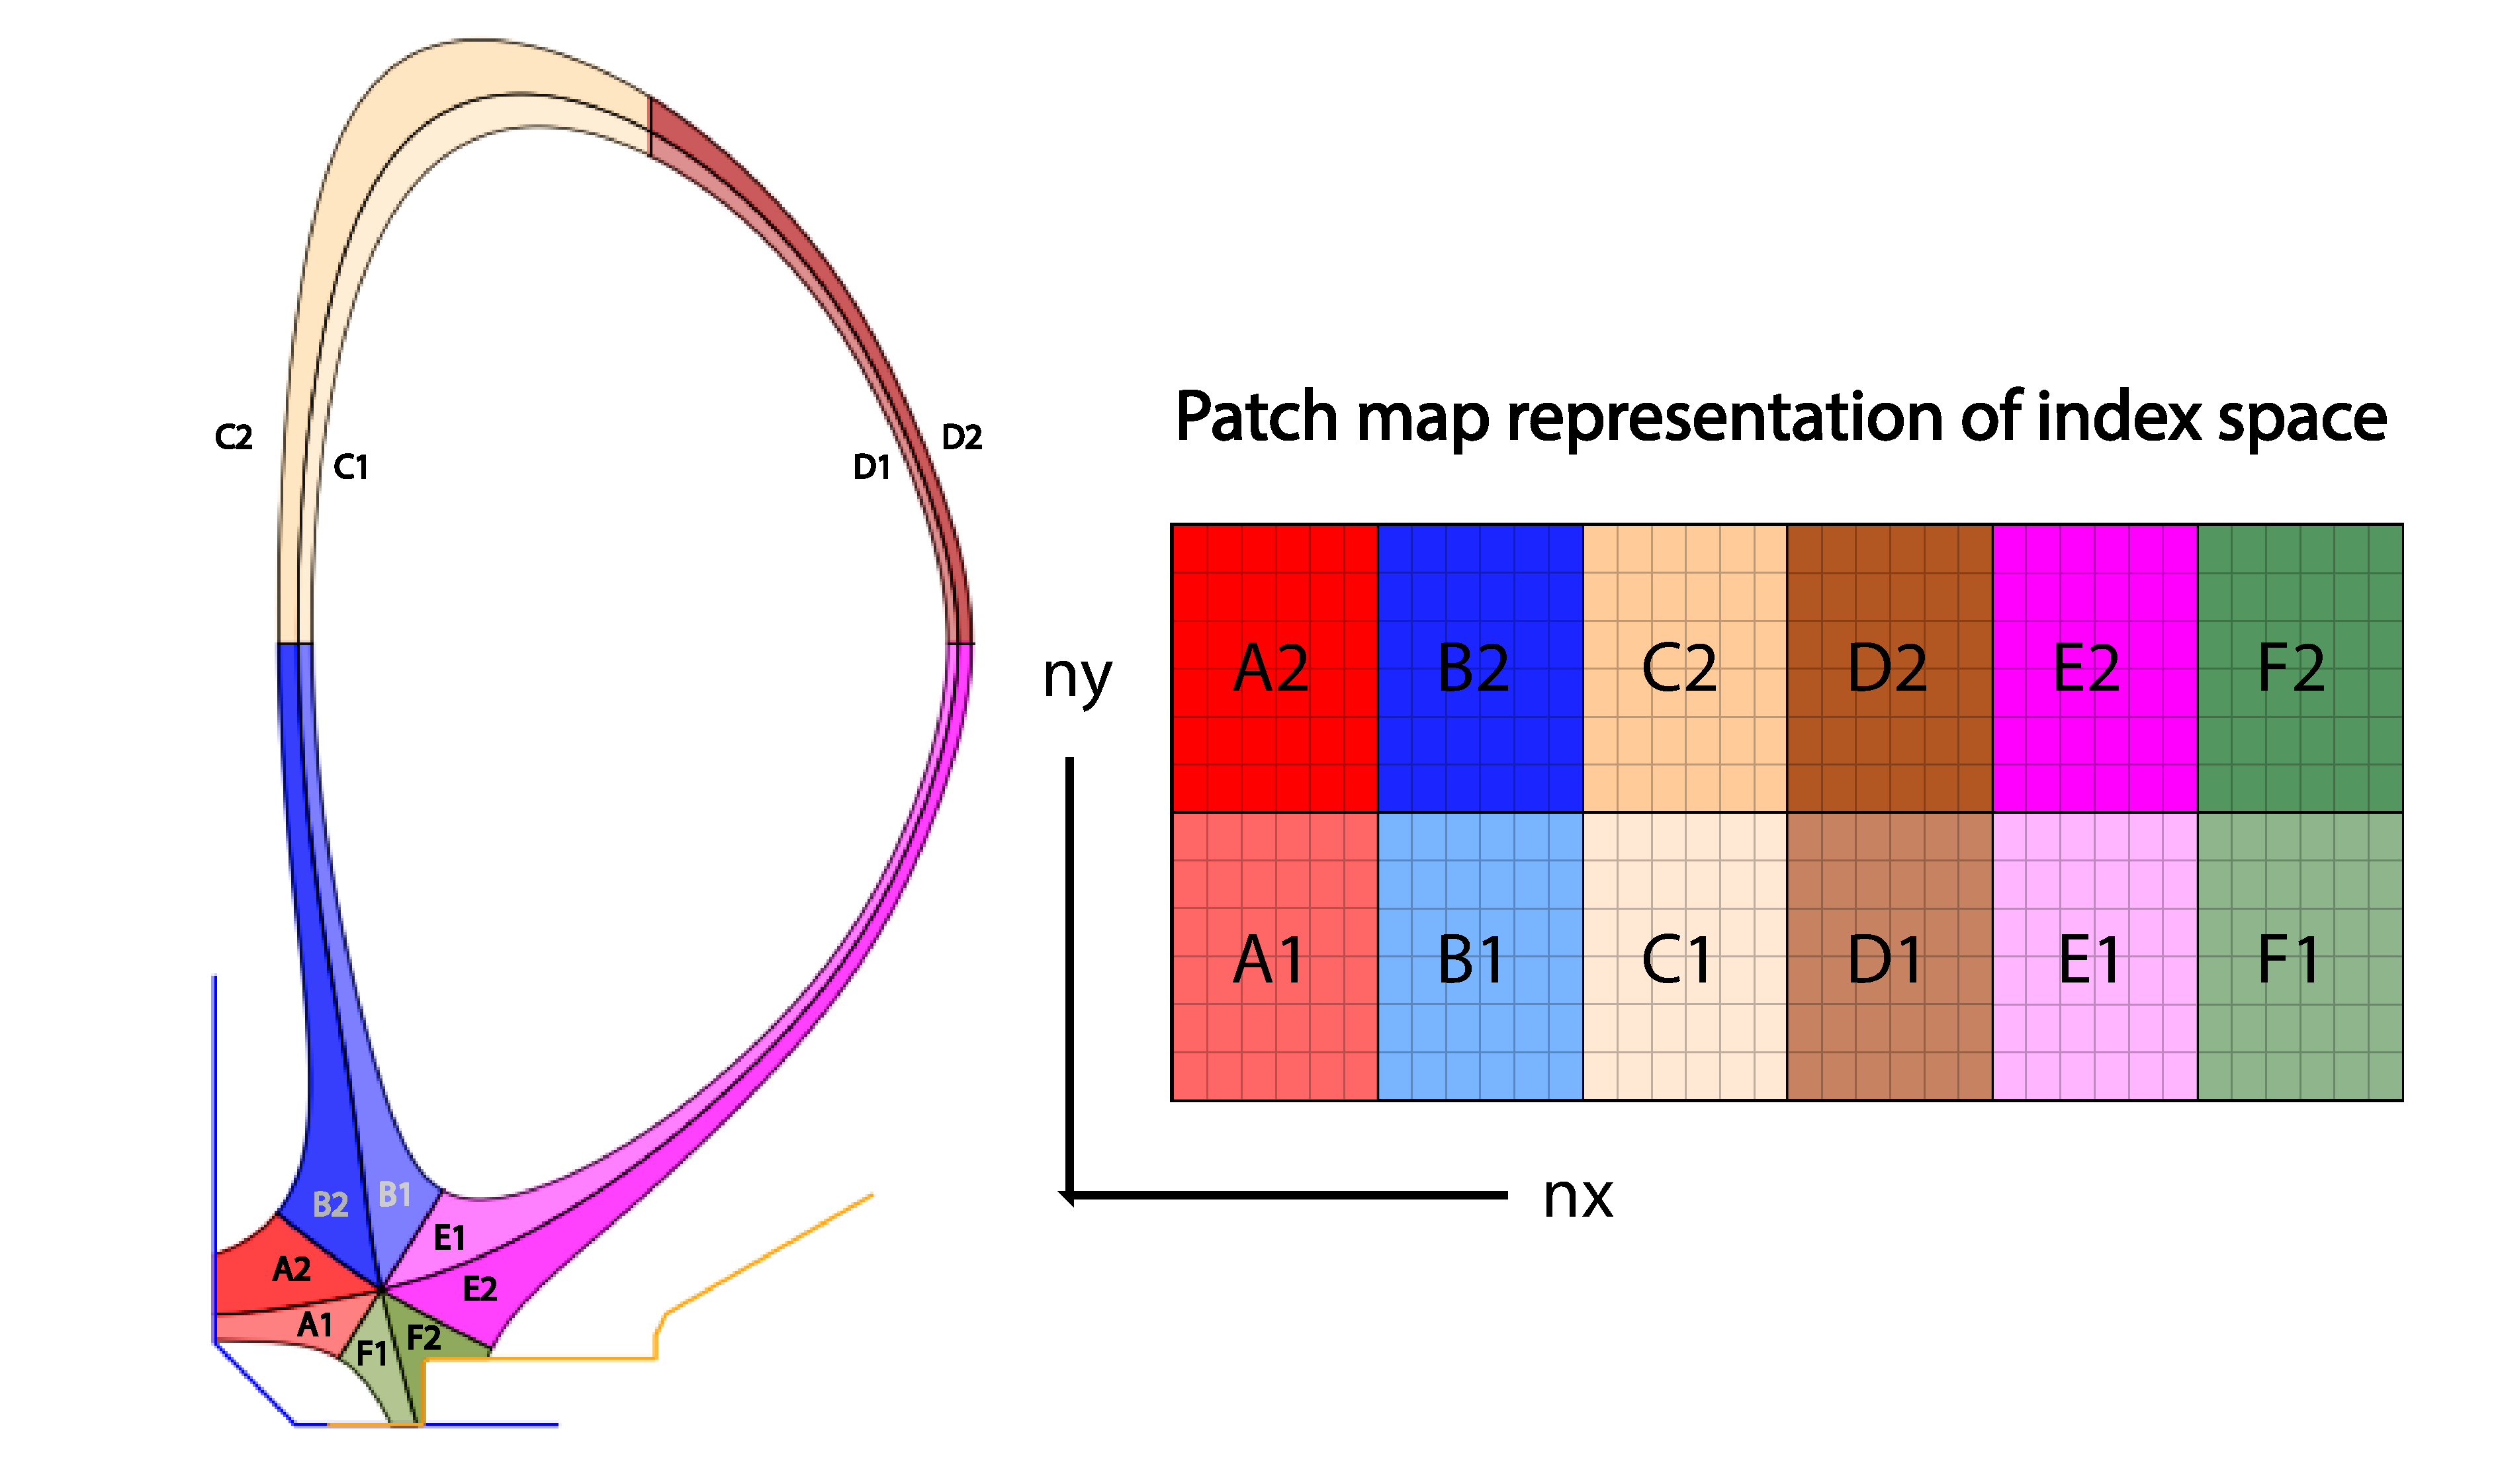
\includegraphics[width=\linewidth]{figures/patch_index_space.pdf}
    \caption{The Patch map of an SNL configuration and it's correspondence to a grid in index space. Individual Patch objects and their region in index space are labeled with a two-character key.}
    \label{fig:snl_patch_index_space}
\end{figure}

\begin{figure}[H]
    \centering
    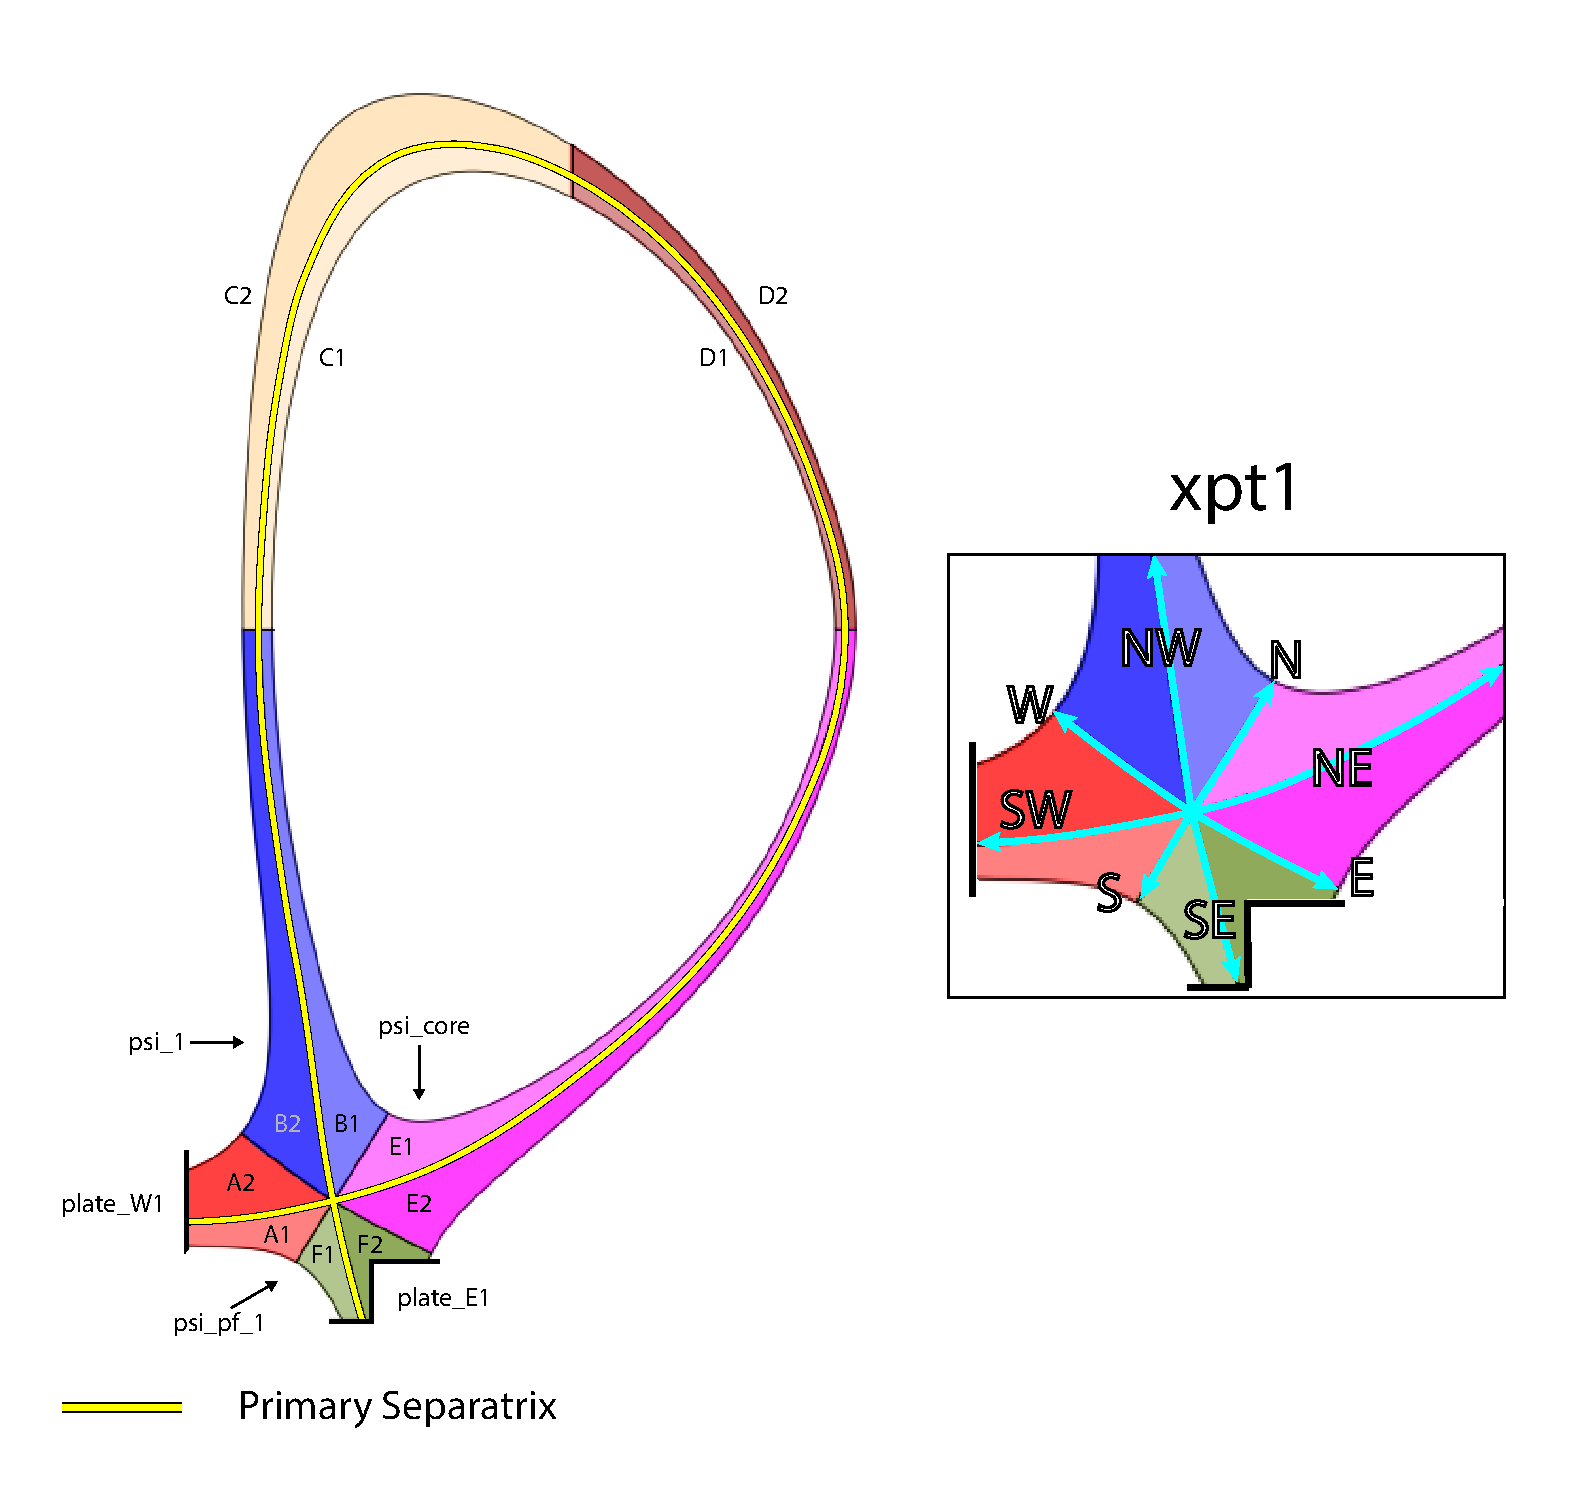
\includegraphics[width=\linewidth]{figures/xpt_1_directions.pdf}
    \caption{An SNL divertor configuration illustrating the primary x-point's N-S-E-W labeling convention.}
    \label{fig:xpt_1_directions}
\end{figure}

\begin{figure}[H]
    \centering
    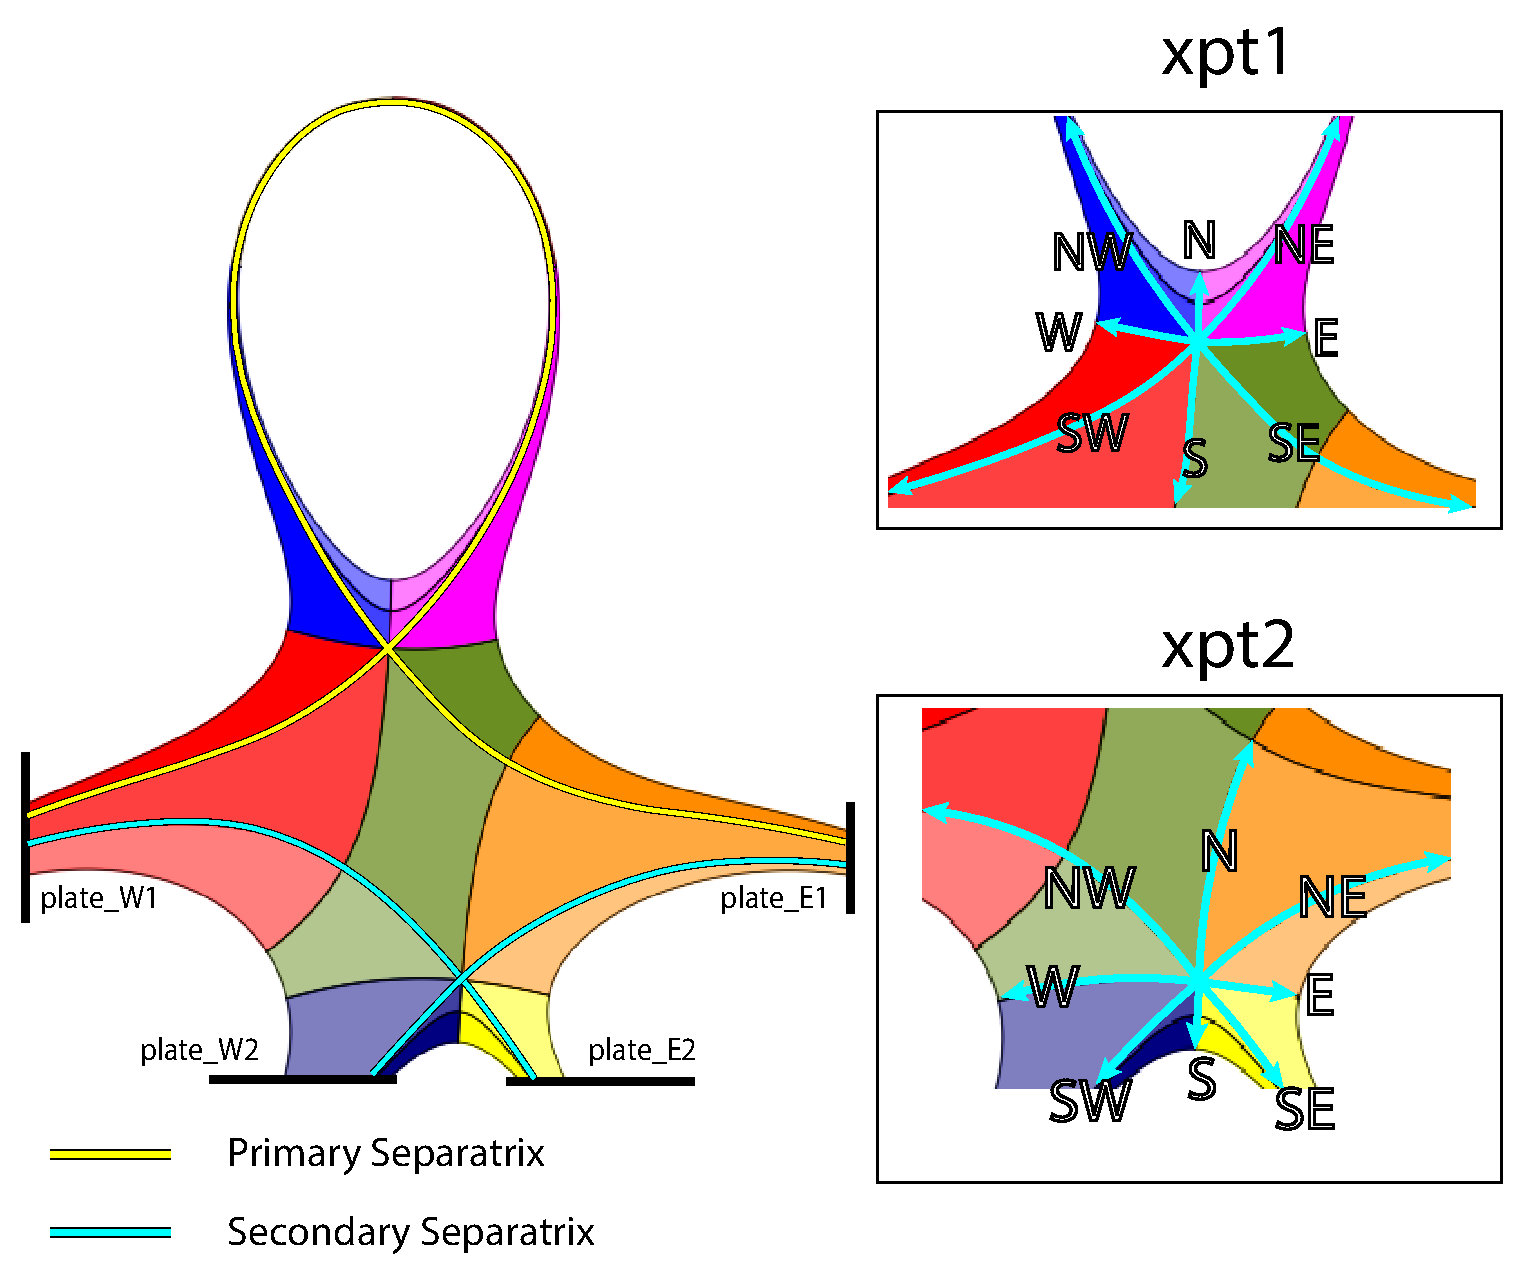
\includegraphics[width=\linewidth]{figures/xpt_2_directions.pdf}
    \caption{An SF75 divertor configuration illustrating the primary x-point and secondary x-point N-S-E-W labeling convention.}
    \label{fig:xpt_2_directions}
\end{figure}

\begin{figure}[H]
    \centering
    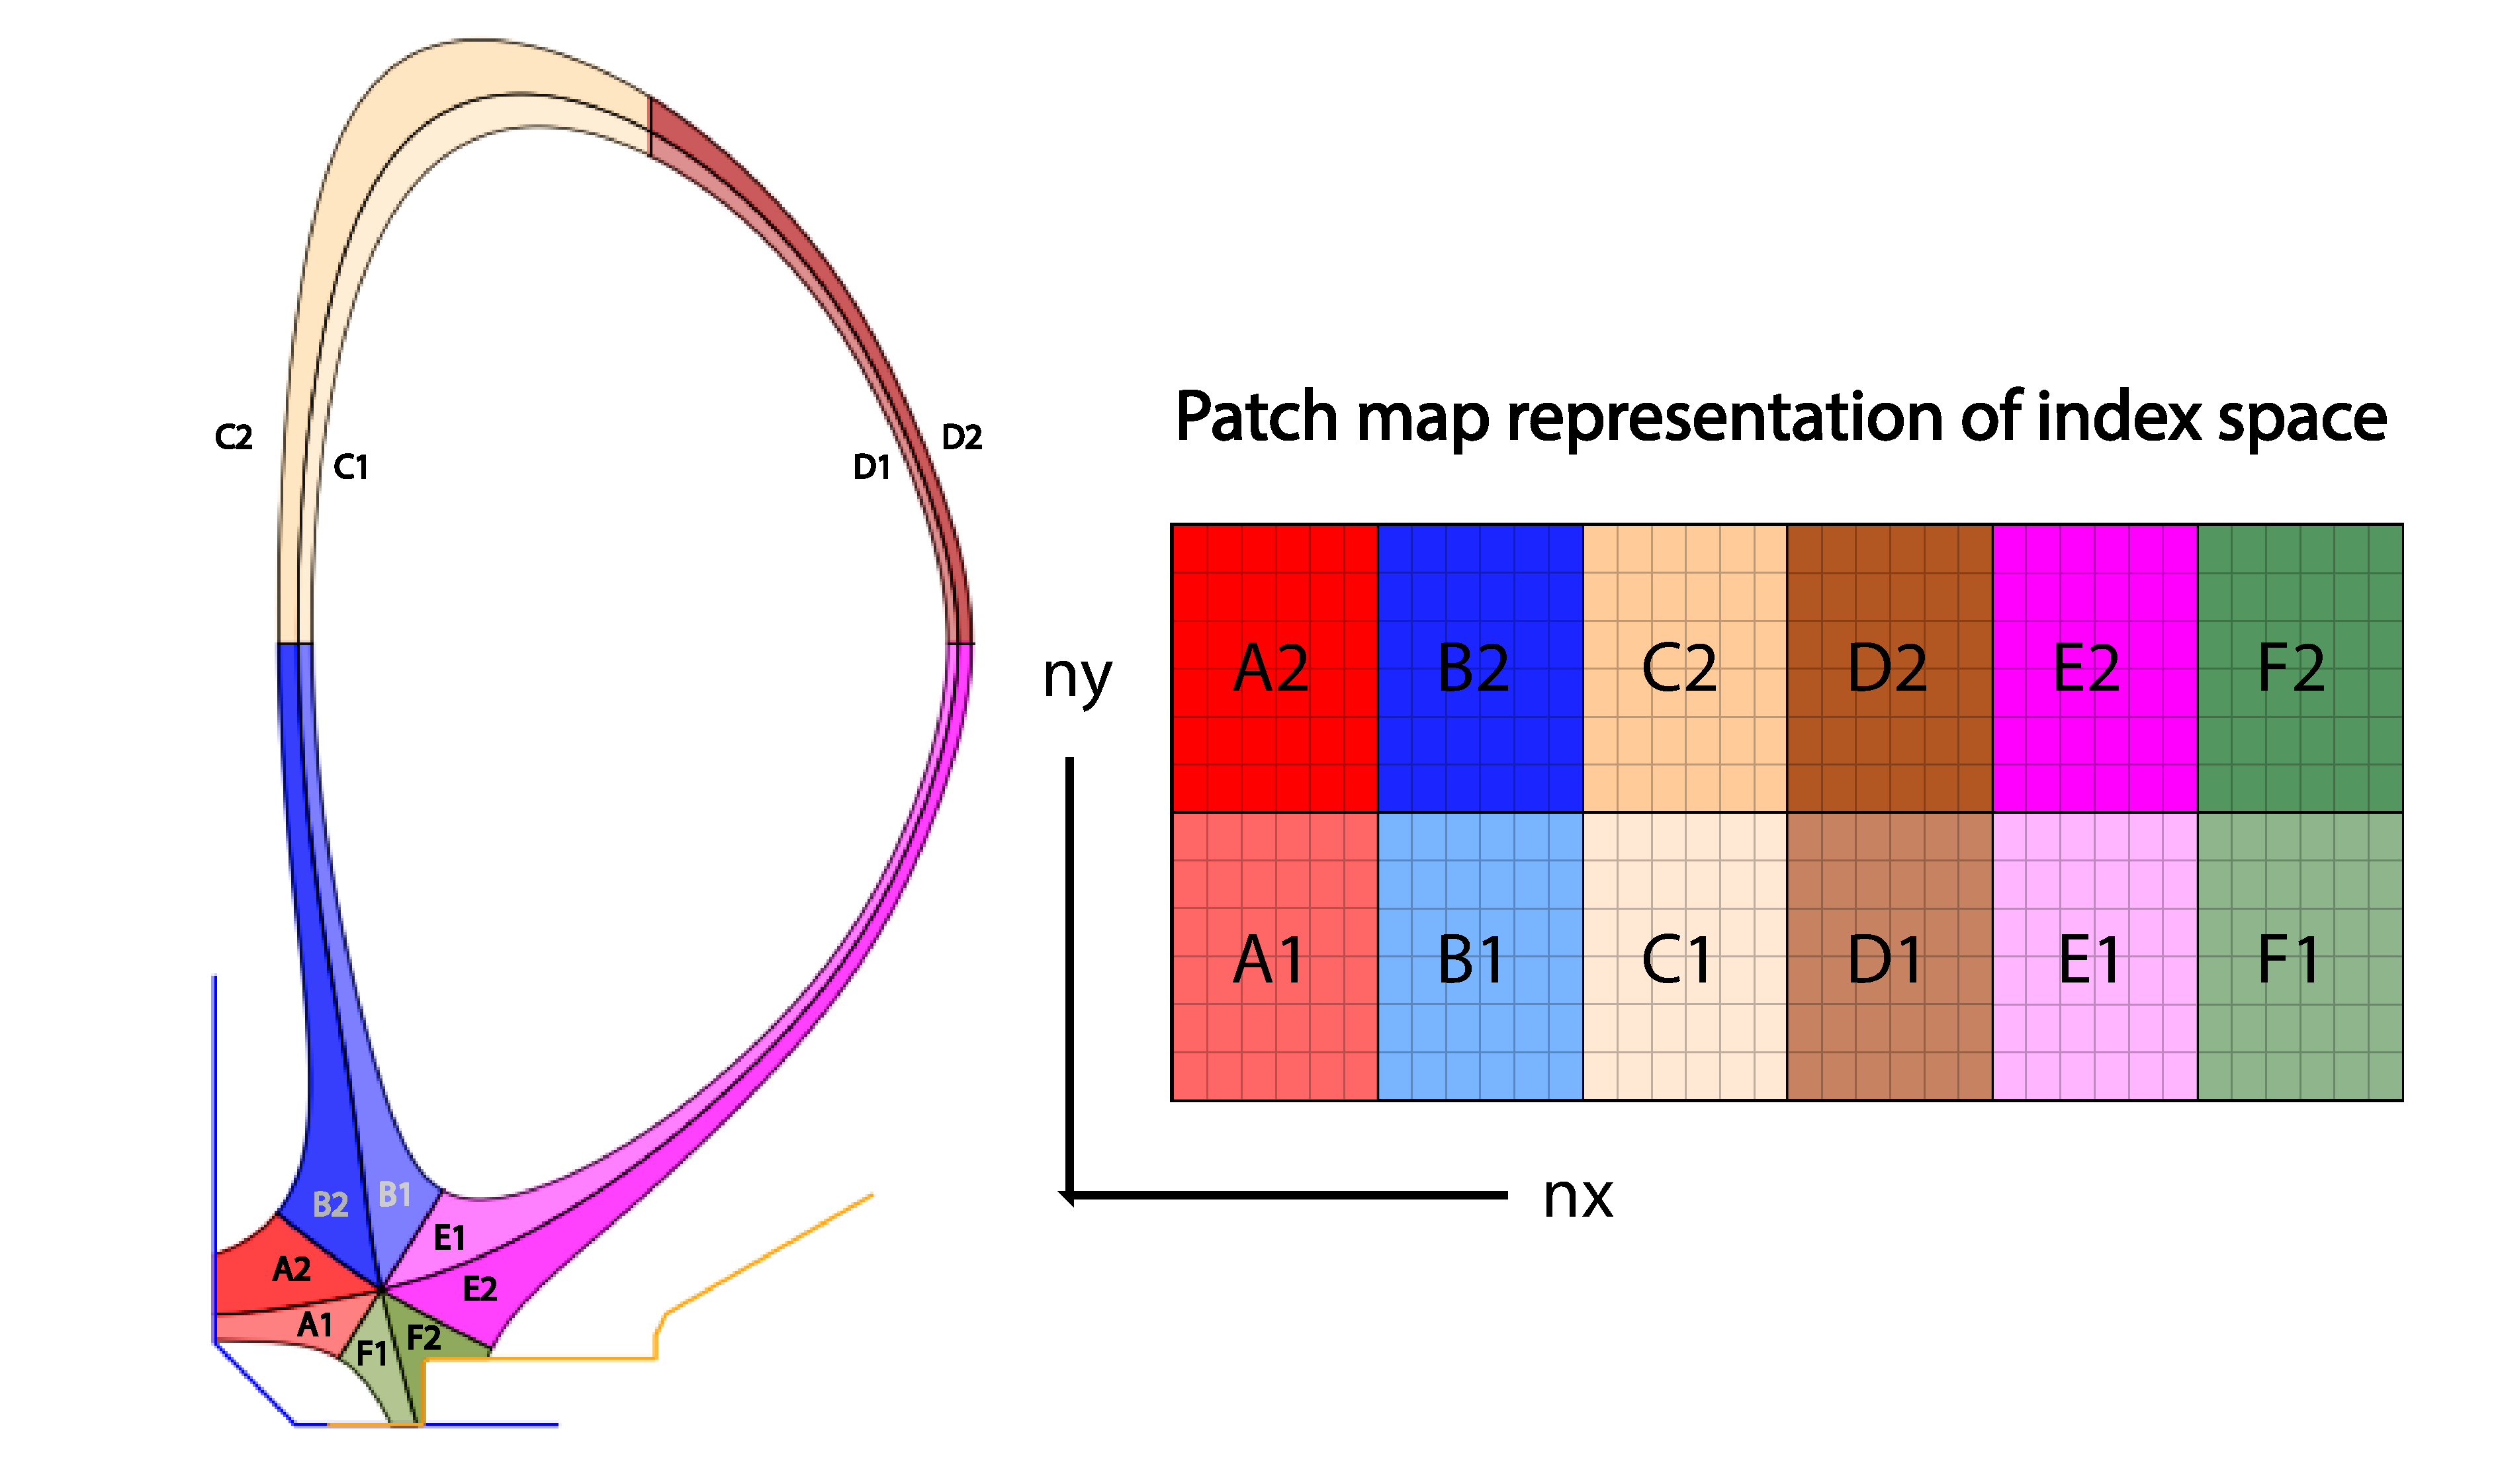
\includegraphics[width=\linewidth]{figures/patch_index_space.pdf}
    \caption{The Patch map of an SNL configuration and it's correspondence to a grid in index space. Individual Patch objects and their region in index space are labeled with a two-character key.}
    \label{fig:snl_patch_index_space}
\end{figure}

\begin{figure}[H]
    \centering
        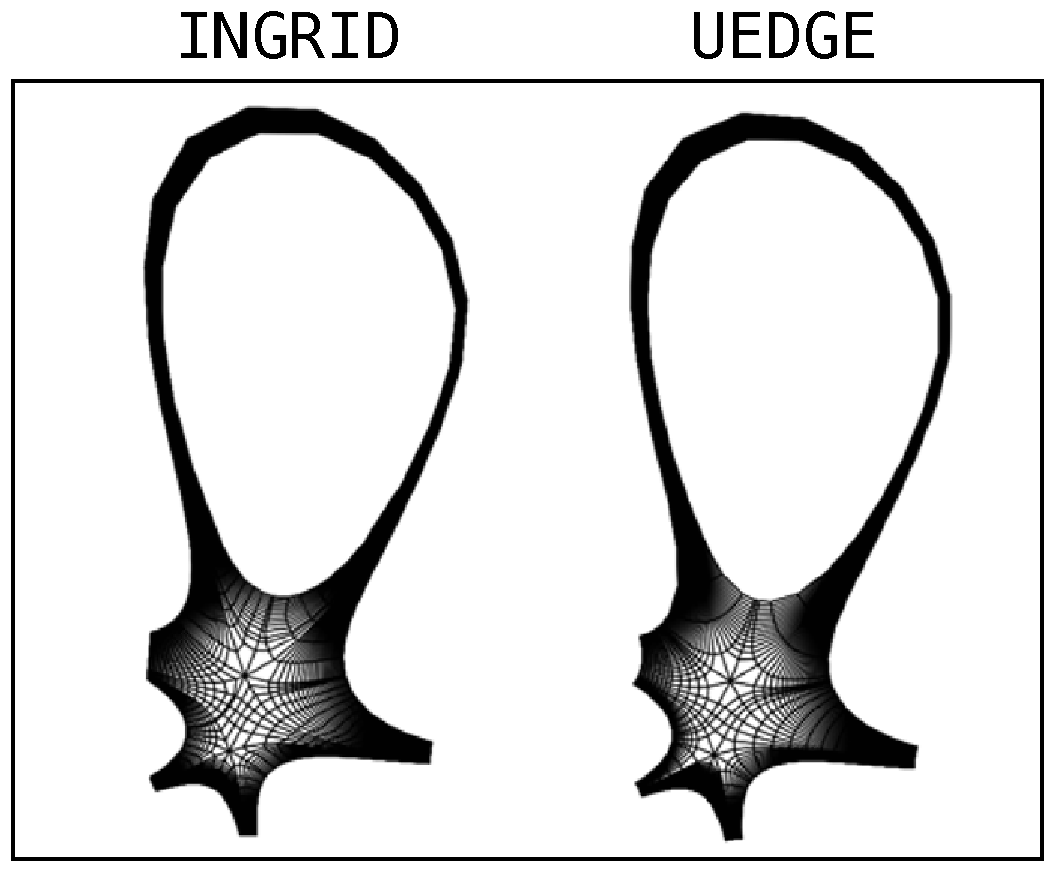
\includegraphics[width=0.9\textwidth]{figures/benchmark/gridue_both.pdf}
        \caption{INGRID and UEDGE generated TCV SF-75 grids.}
        \label{fig:ingrid_grid}
\end{figure}
\begin{figure}[H]
    \centering
        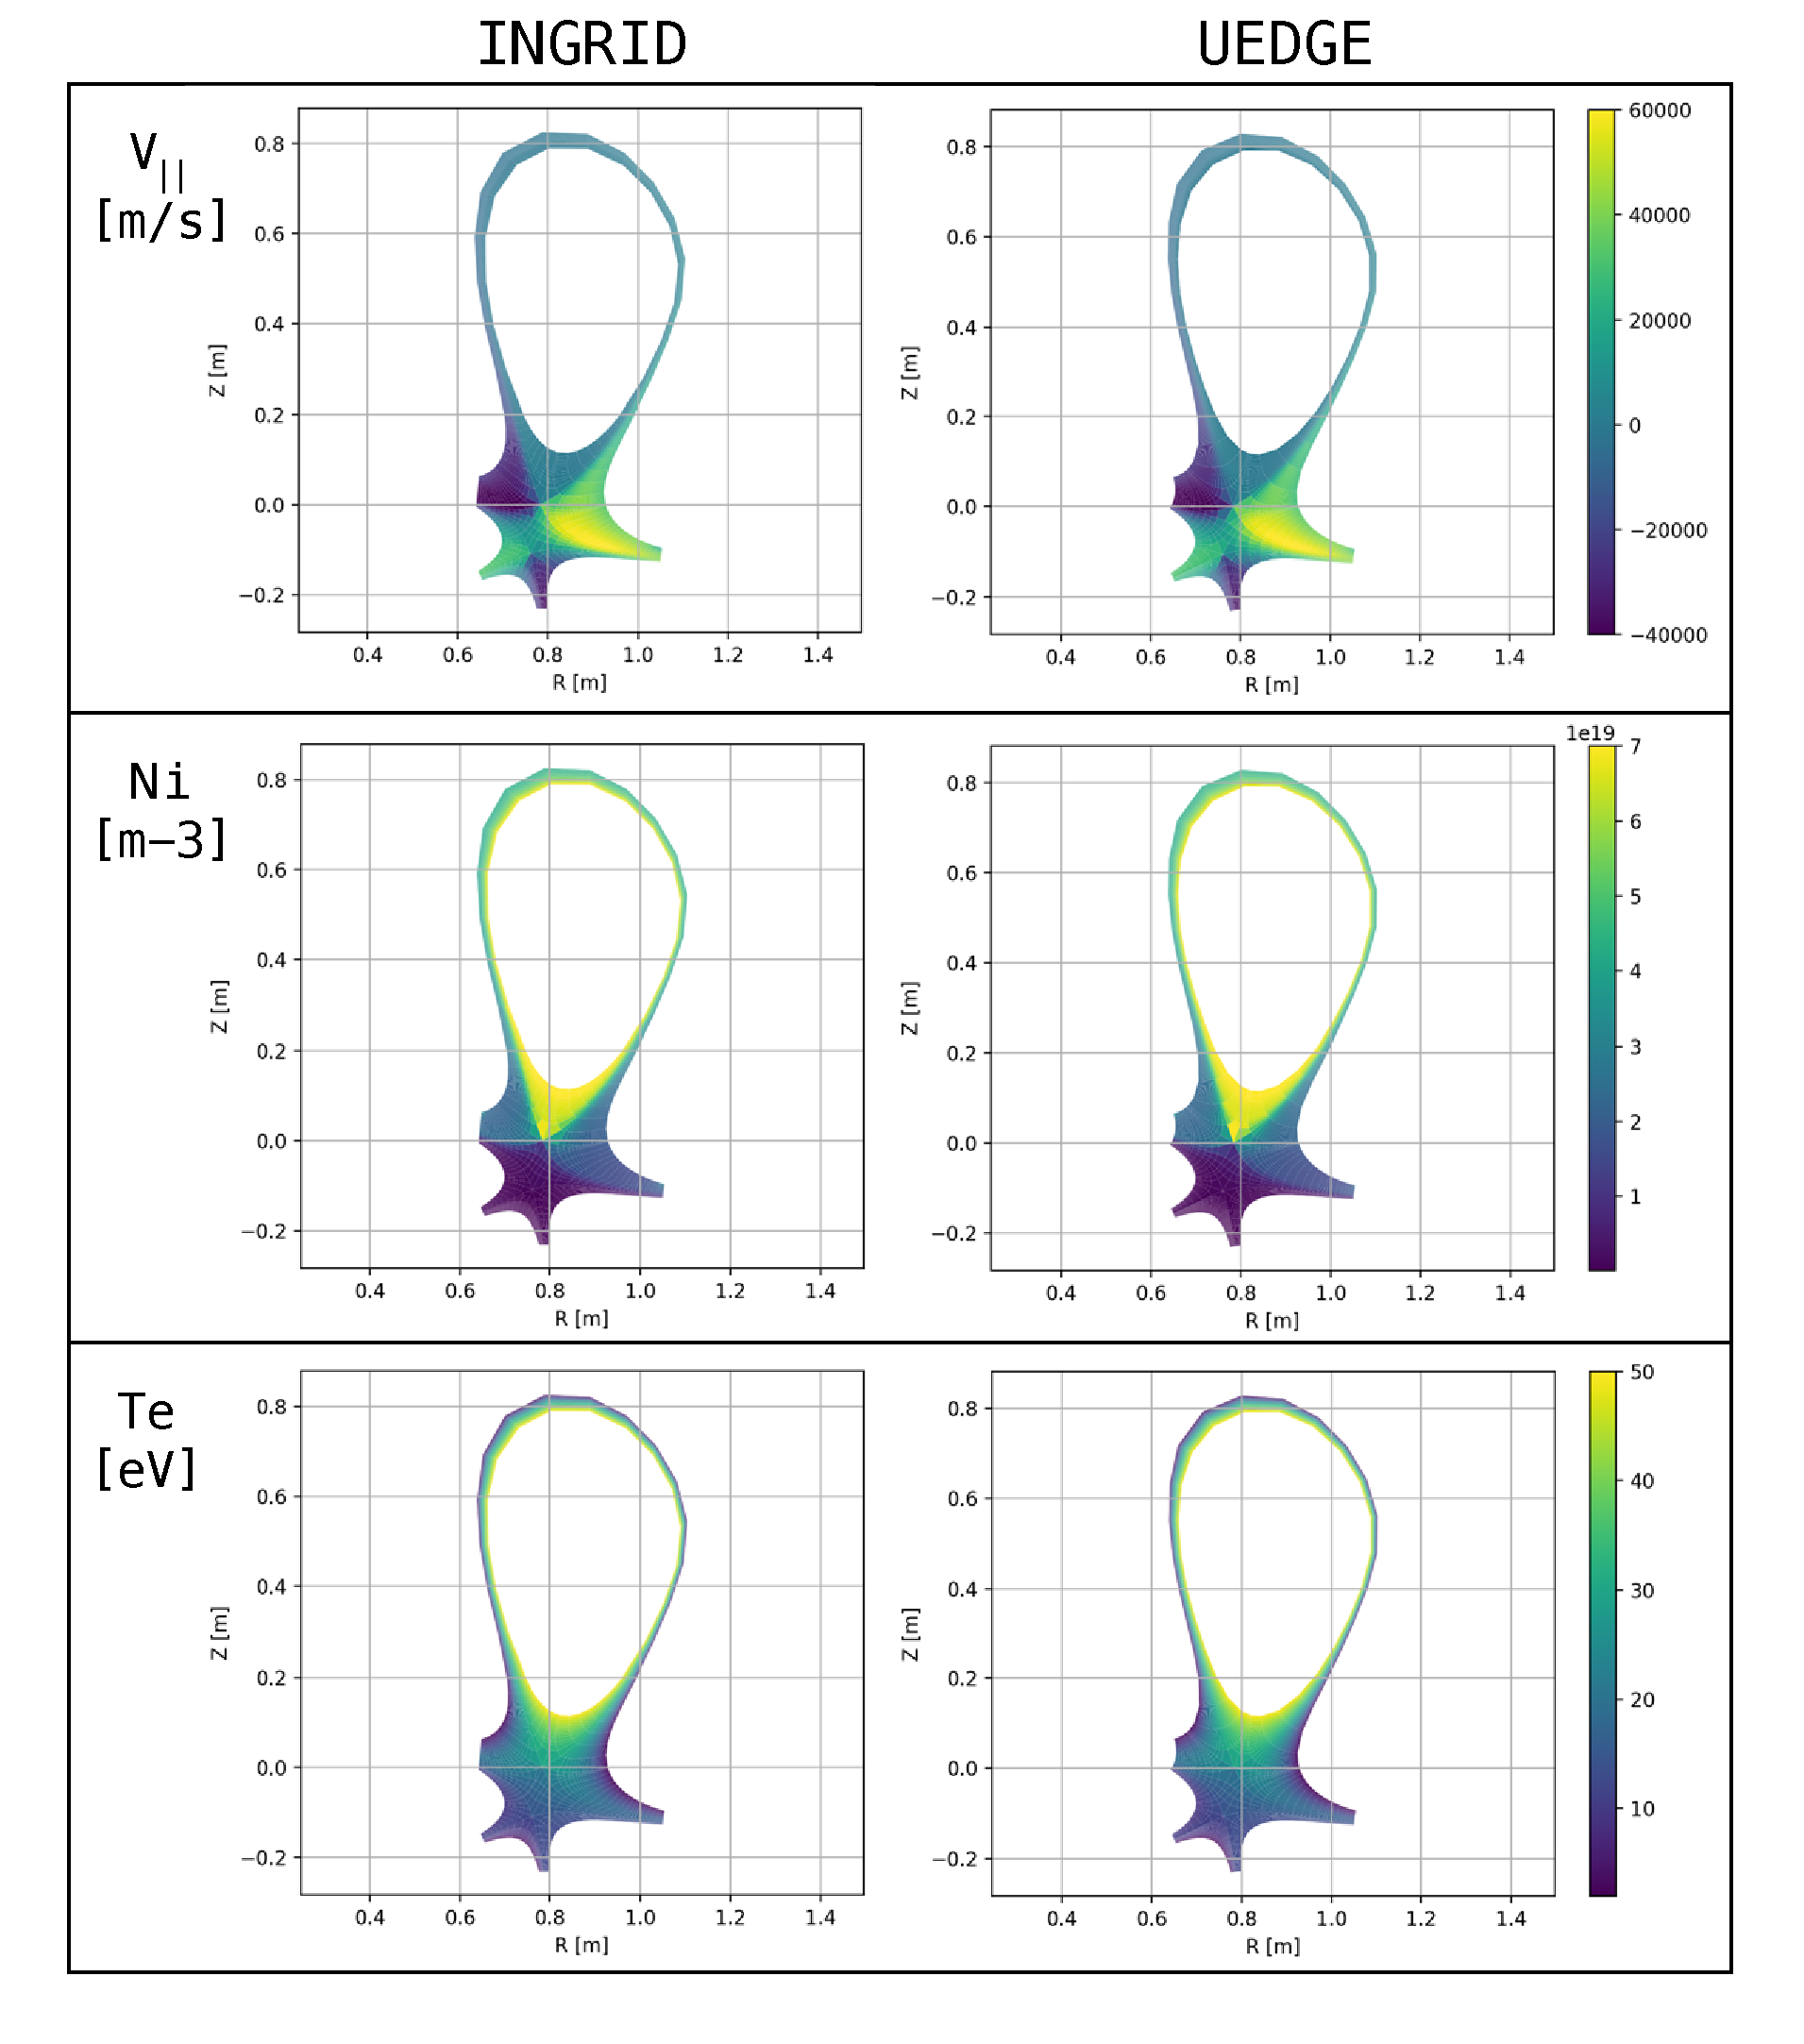
\includegraphics[width=\textwidth]{figures/benchmark/BenchmarkCollection.pdf}
        \caption{A collection of UEDGE simulations run on INGRID and UEDGE generated grids.}
        \label{fig:benchmark_collection}
\end{figure}

\section{Supported divertor configurations}
\begin{figure}[H]
    \centering
        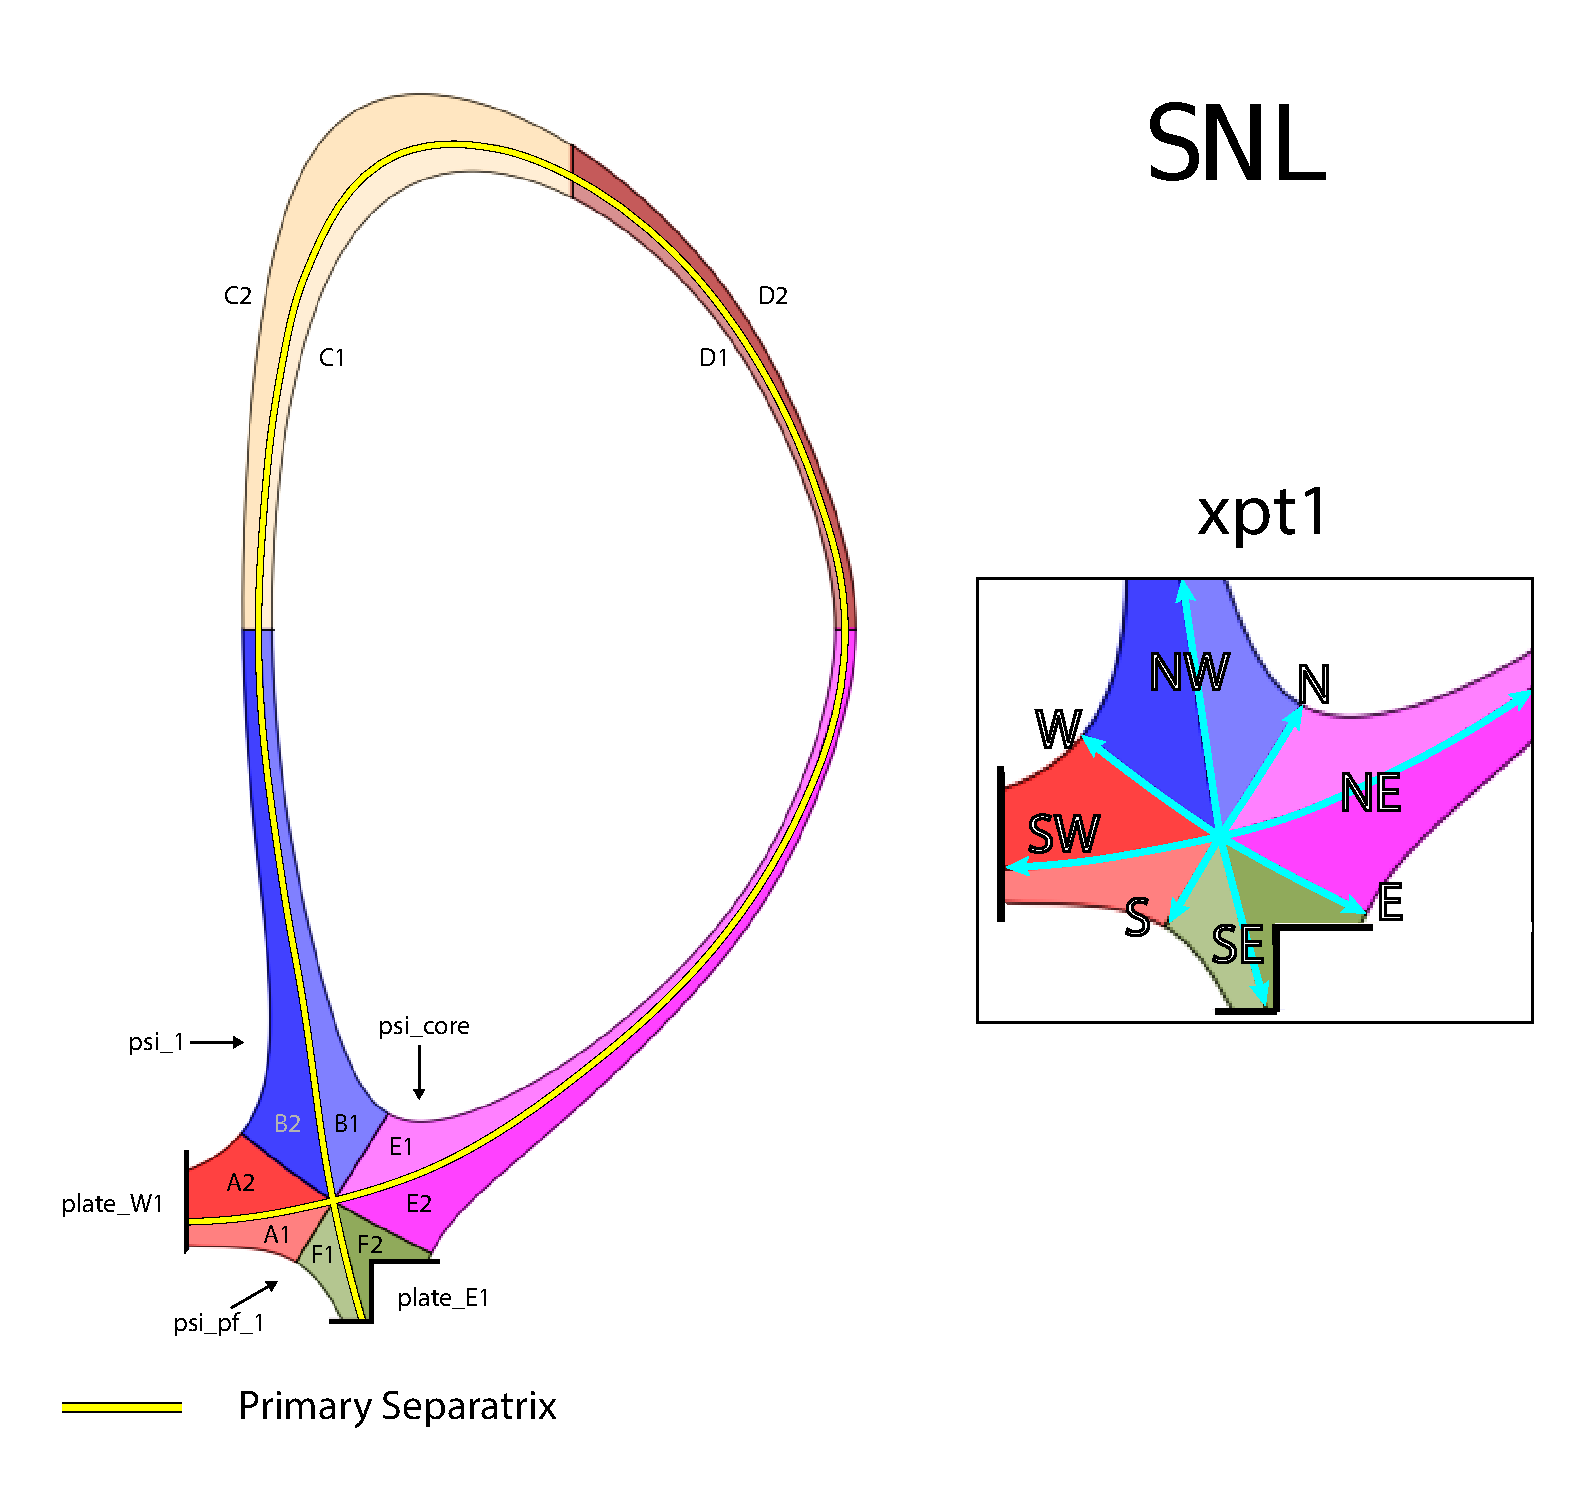
\includegraphics[width=\textwidth]{figures/configurations/SNL_collection.pdf}
        \caption{SNL Patch map}
        \label{fig:snl_patch_map}
\end{figure}
\begin{figure}[H]
    \centering
        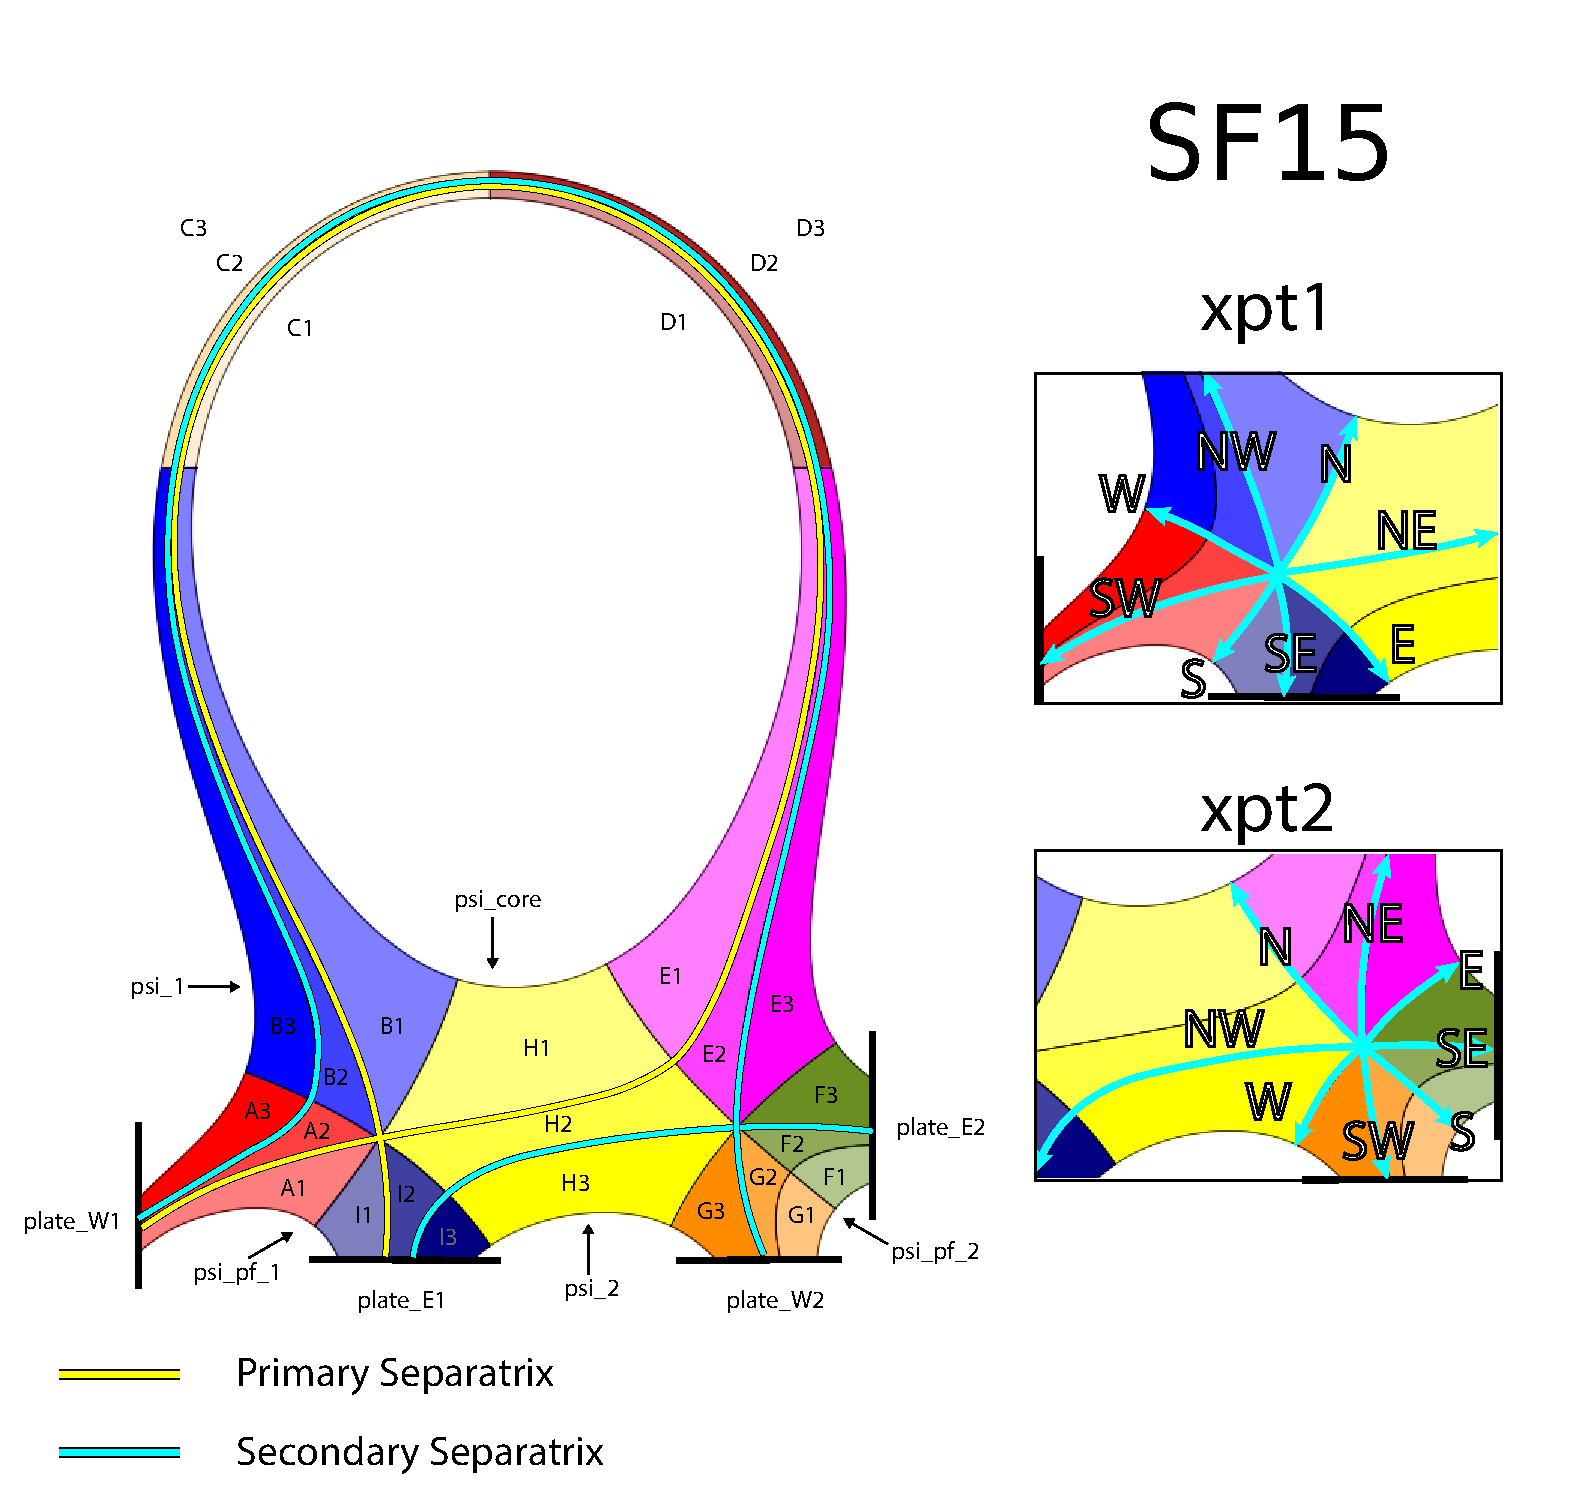
\includegraphics[width=\textwidth]{figures/configurations/SF15_collection.pdf}
        \caption{SF15 Patch map}
        \label{fig:sf15_patch_map}
\end{figure}
\begin{figure}[H]
    \centering
        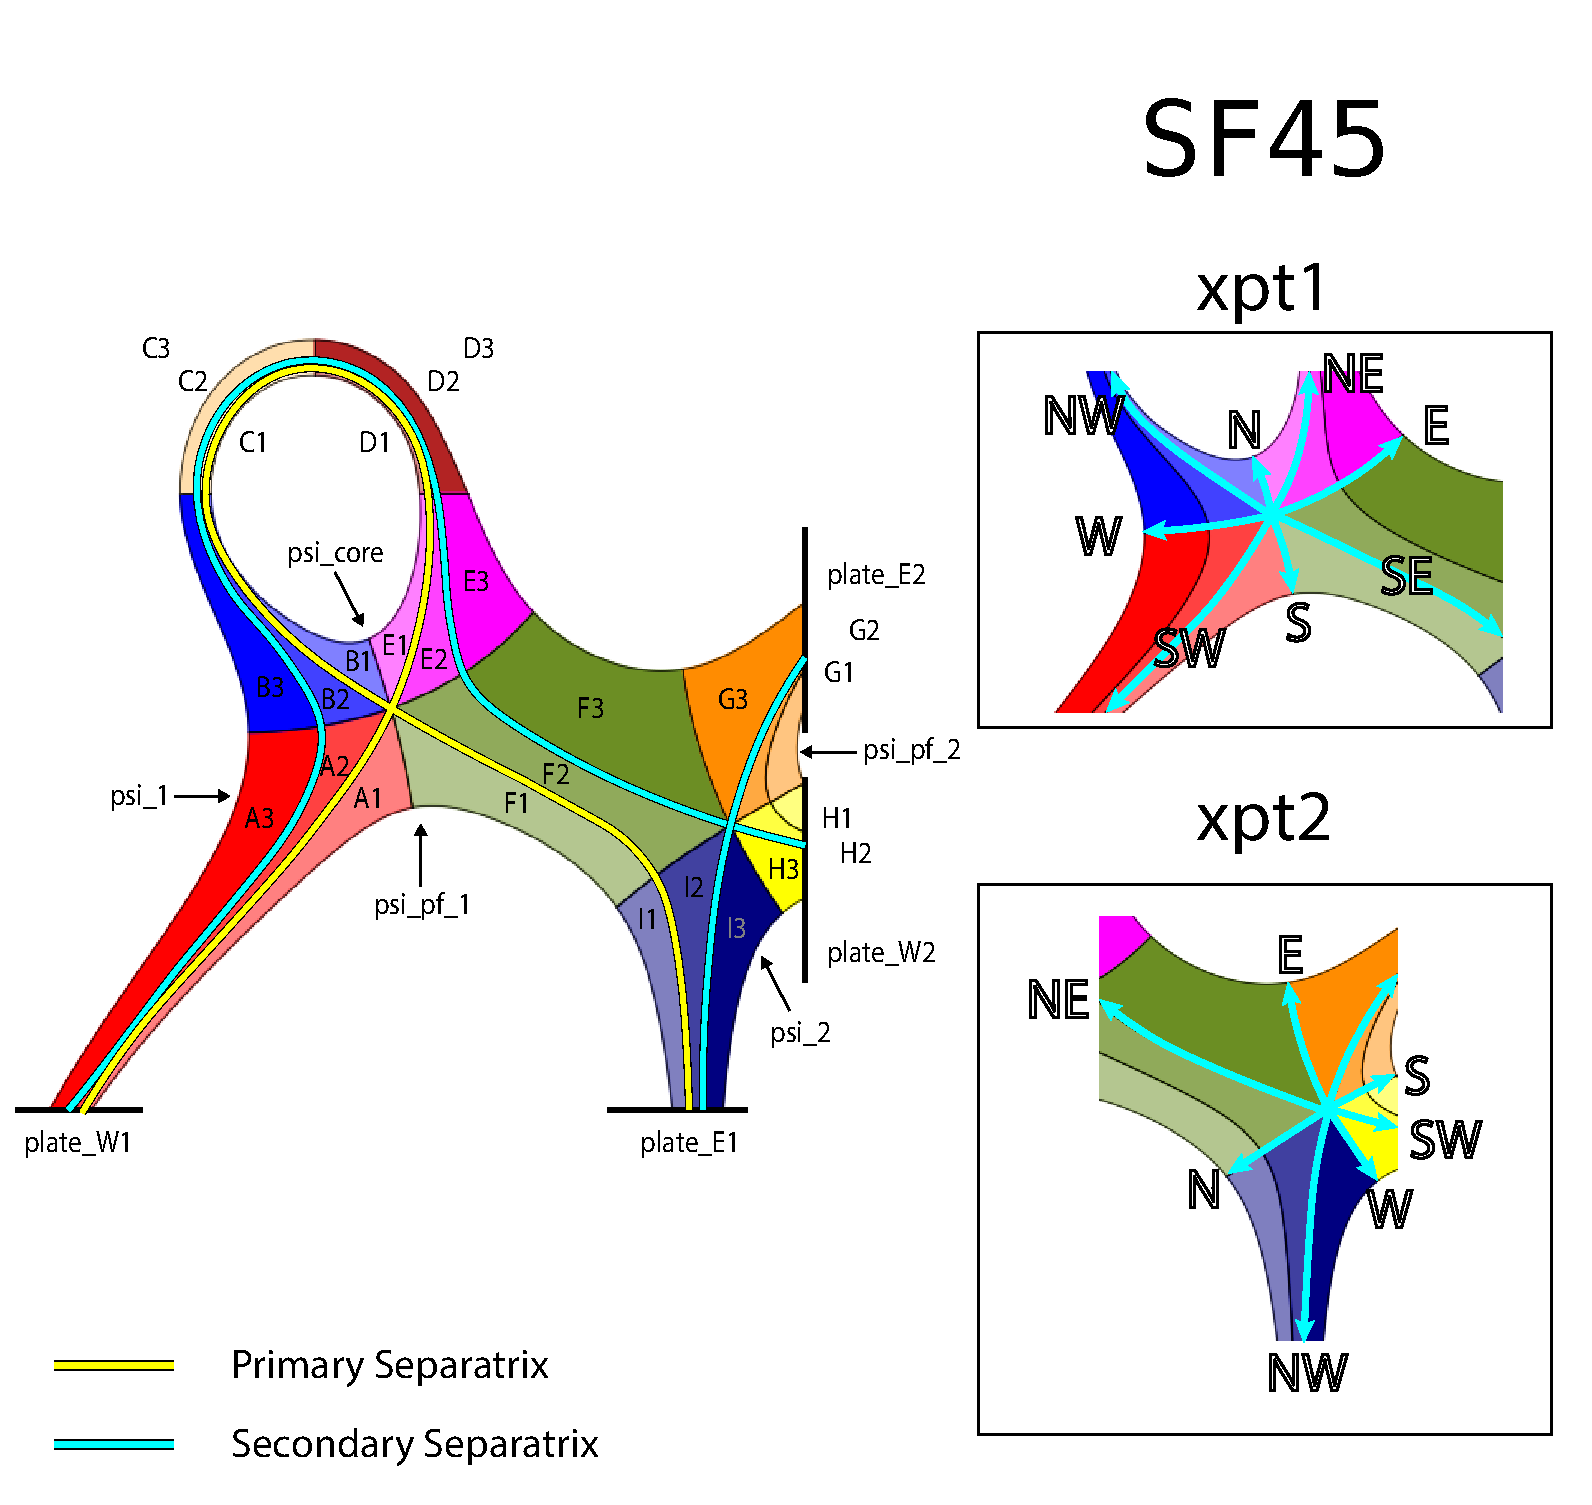
\includegraphics[width=1.05\textwidth]{figures/configurations/SF45_collection.pdf}
        \caption{SF45 Patch map}
        \label{fig:sf45_patch_map}
\end{figure}
\begin{figure}[H]
    \centering
        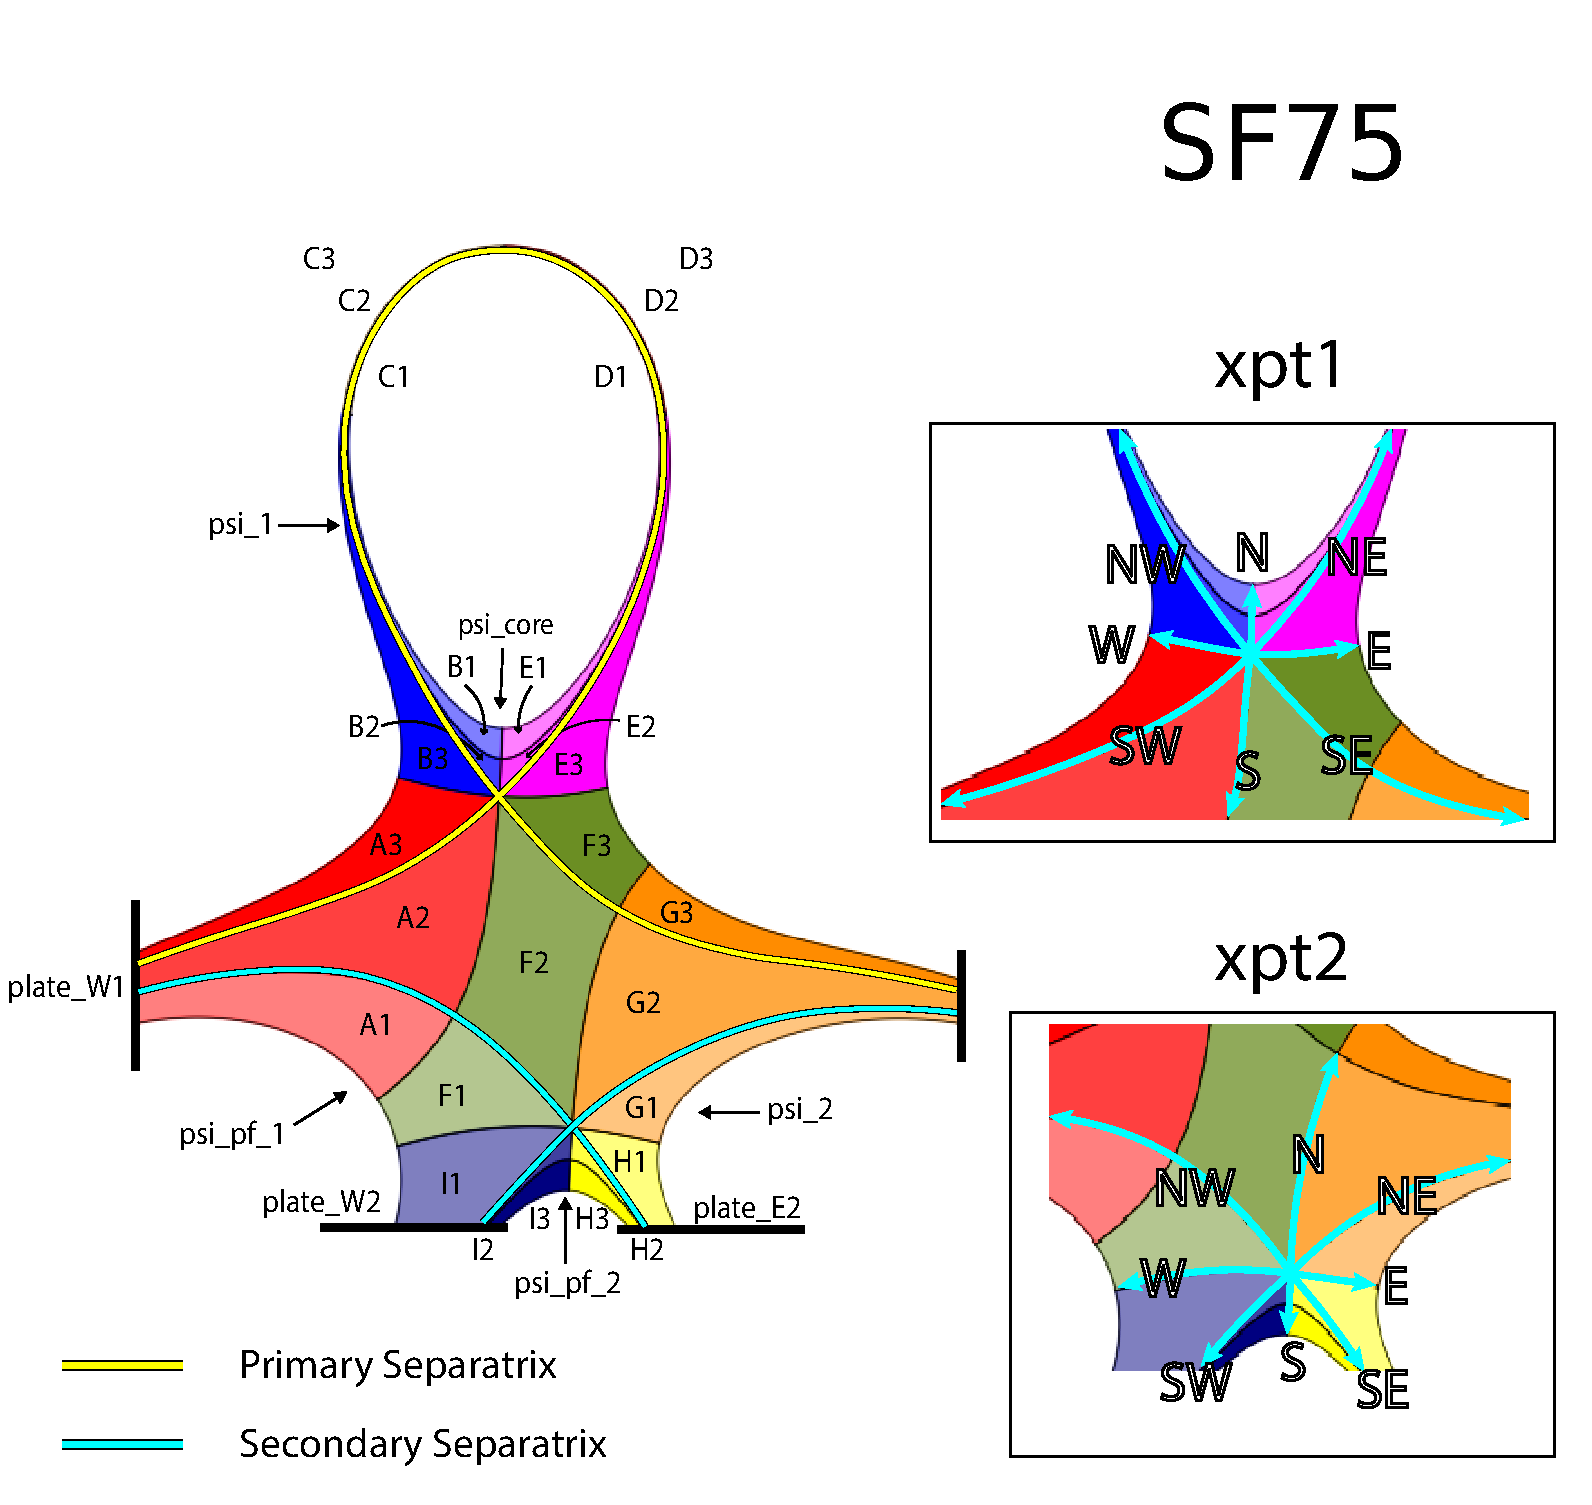
\includegraphics[width=\textwidth]{figures/configurations/SF75_collection.pdf}
        \caption{SF75 Patch map}
        \label{fig:sf75_patch_map}
\end{figure}
\begin{figure}[H]
    \centering
        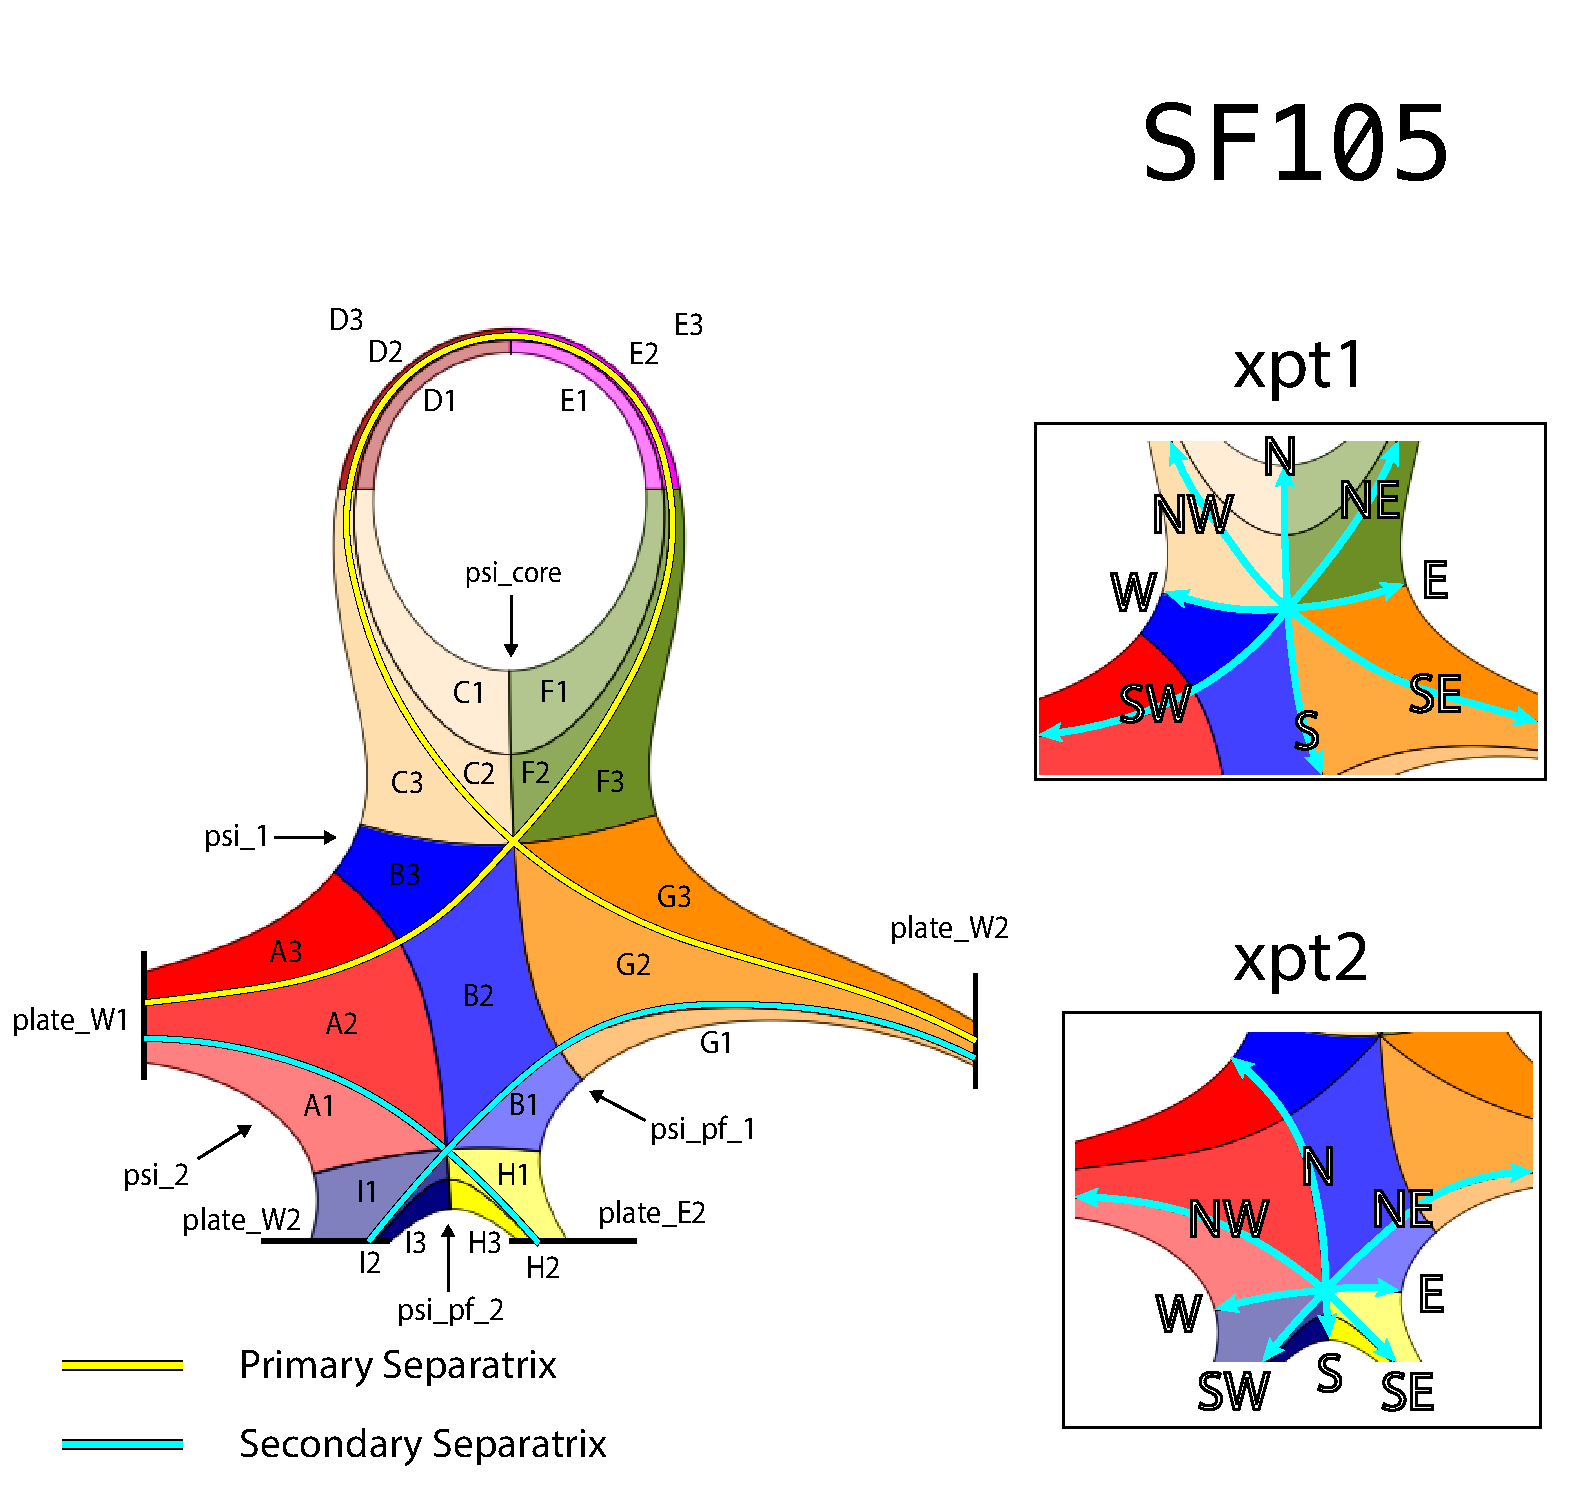
\includegraphics[width=\textwidth]{figures/configurations/SF105_collection.pdf}
        \caption{SF105 Patch map}
        \label{fig:sf105_patch_map}
\end{figure}
\begin{figure}[H]
    \centering
        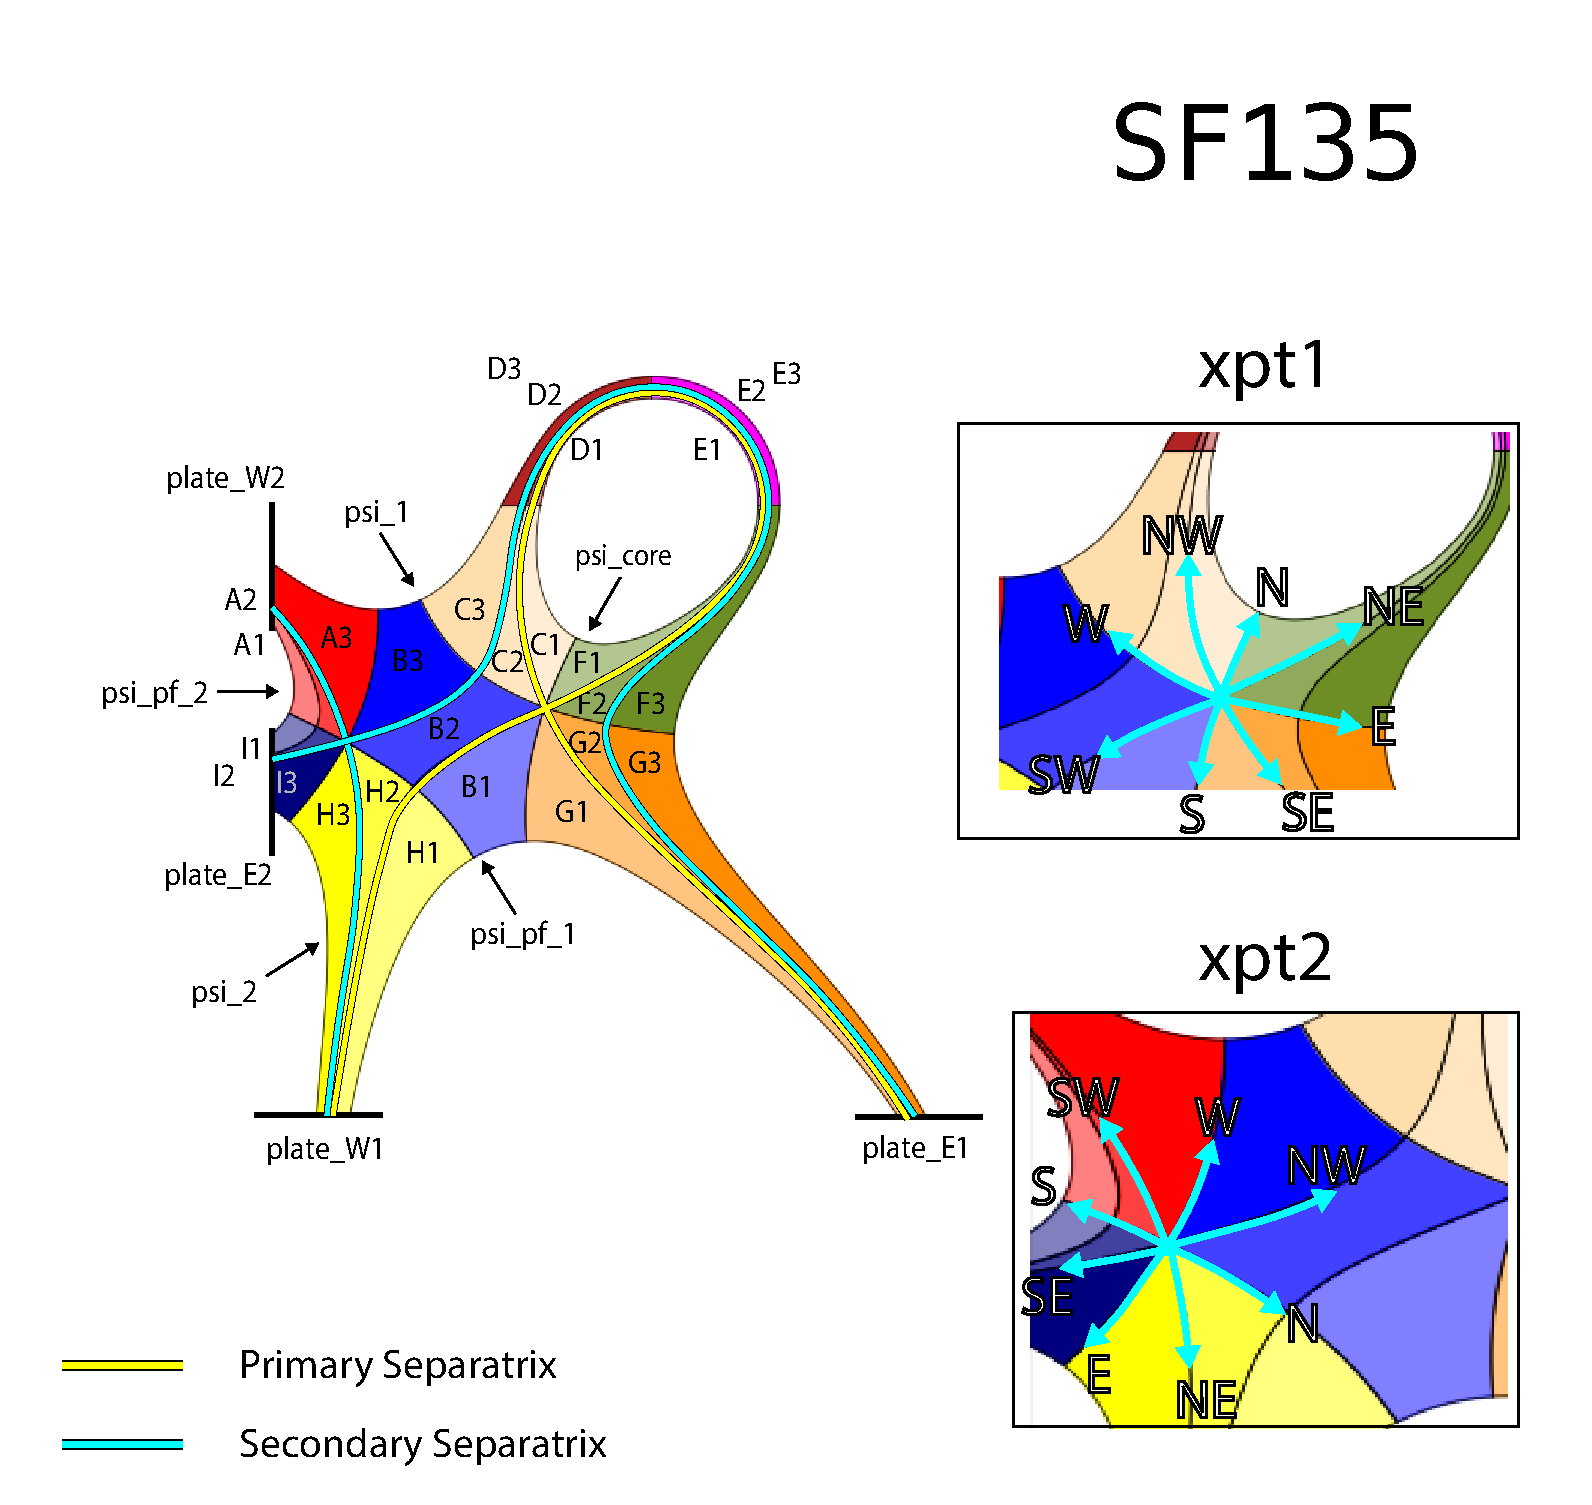
\includegraphics[width=1.05\textwidth]{figures/configurations/SF135_collection.pdf}
        \caption{SF135 Patch map}
        \label{fig:sf135_patch_map}
\end{figure}
\begin{figure}[H]
    \centering
        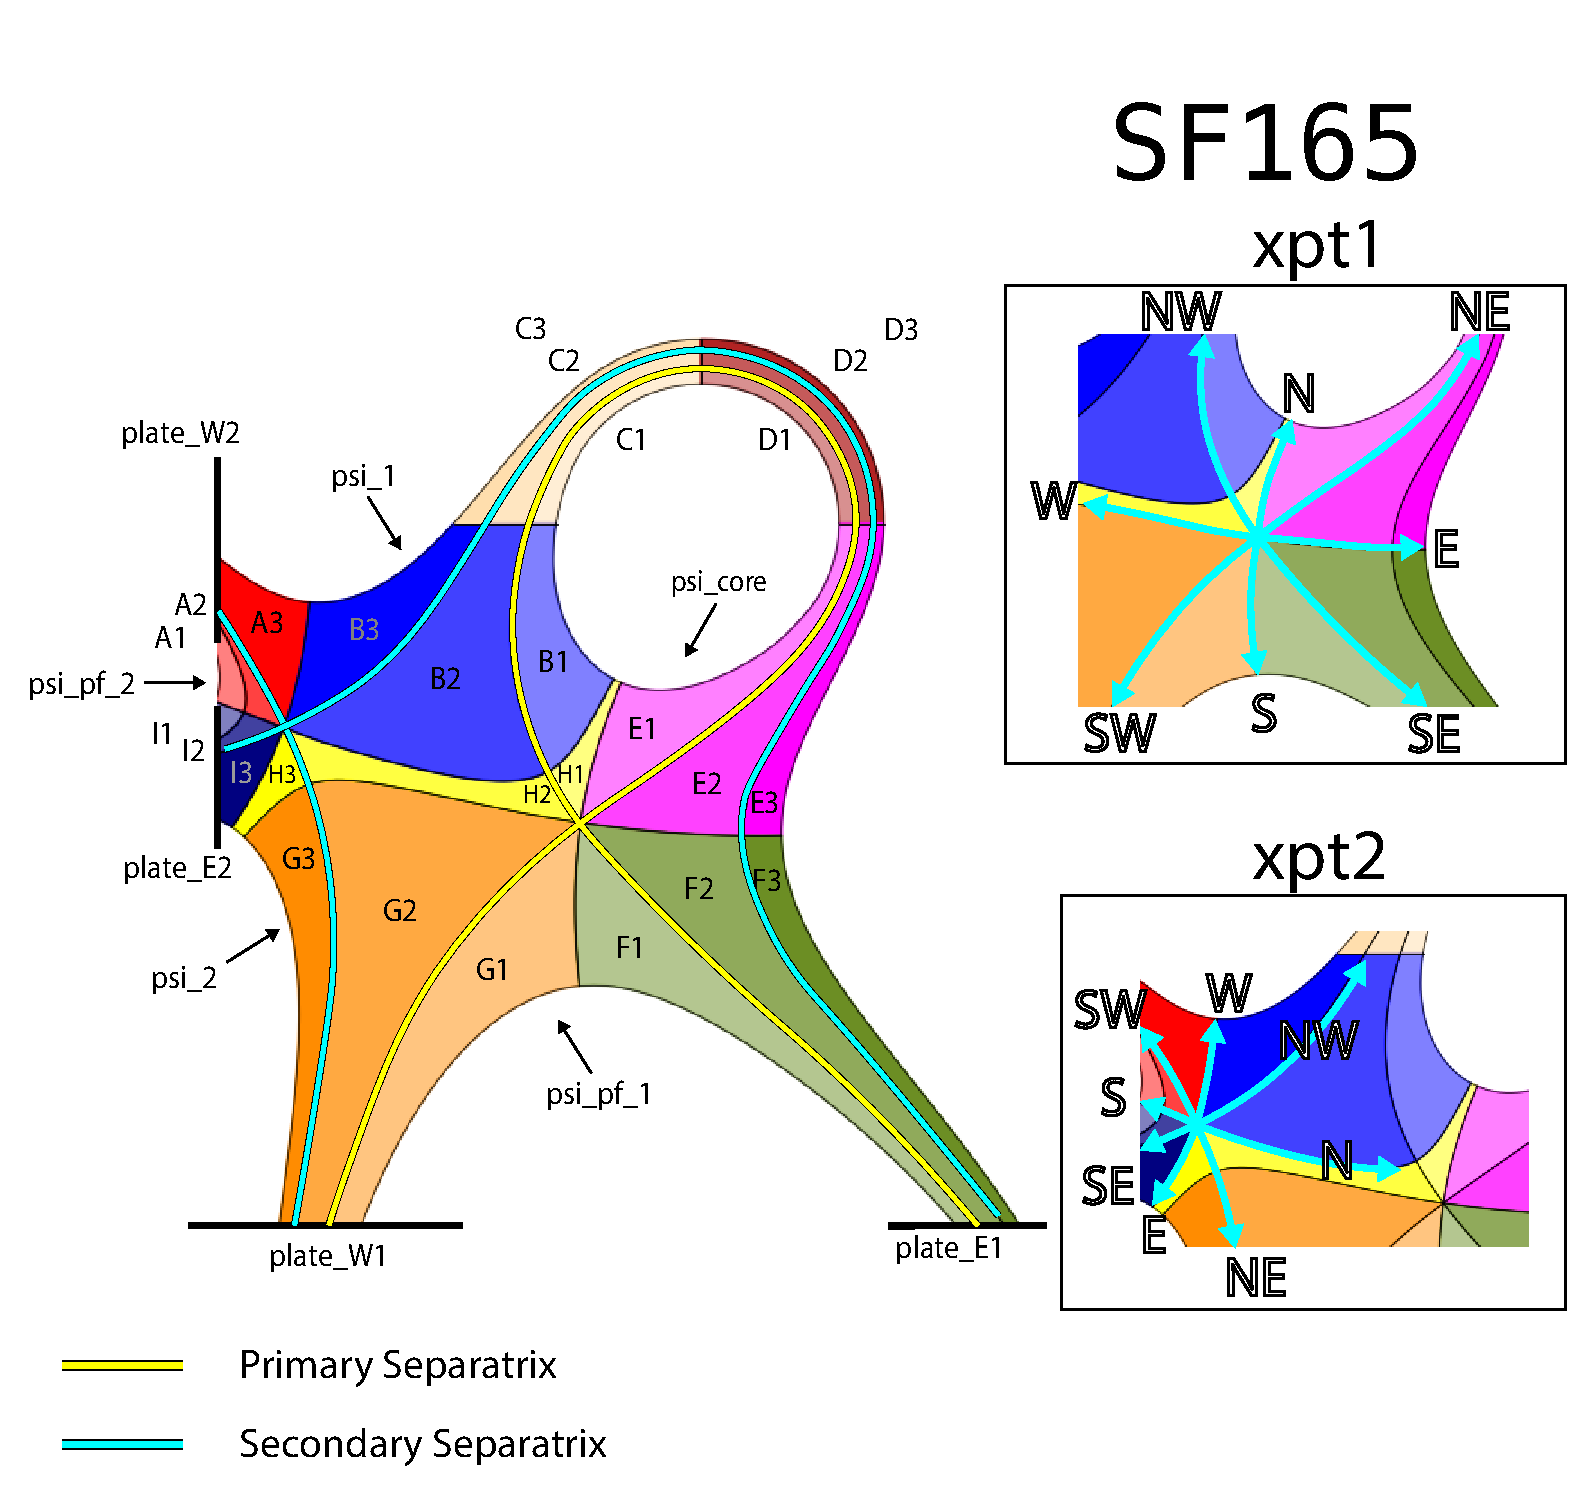
\includegraphics[width=\textwidth]{figures/configurations/SF165_collection.pdf}
        \caption{SF165 Patch map}
        \label{fig:sf165_patch_map}
\end{figure}


\end{document}
